%=====使用mcmthesis数模美赛模板======
\documentclass{mcmthesis}
%=============================

%=====mcmthesis模板设置===========================
\mcmsetup{CTeX = FALSE,   
        tcn = 1924678, problem =C,
        sheet = true, titleinsheet = true, keywordsinsheet = false,
        titlepage = false, abstract = true}
%=====keywords手动输入,无标题页=====================
%=============================================

%=====补充宏包=========================
\usepackage{palatino}
\usepackage{float}
\usepackage{graphicx}
\usepackage{subfigure}
\usepackage{chngpage}
\usepackage{threeparttable}
\usepackage[numbers,sort&compress]{natbib}
\usepackage{titlesec}
%===================================

%=====设置列表格式================================
\usepackage{enumerate}
\usepackage{enumitem}
\setlist[enumerate,1]{label=(\arabic*),font=\textup,
leftmargin=3.4em,labelsep=1.5mm,topsep=0mm,itemsep=-0.8mm}
\setlist[enumerate,2]{label=(\alph*),font=\textup, 
leftmargin=1.6em,labelsep=1.5mm,topsep=0mm,itemsep=-0.8mm}
%=====修改格式需每次使用前单独设置=====================
%=============================================

%=====设置公式图表编号格式=============================
\newcounter{rowno}
\numberwithin{equation}{section}
\numberwithin{figure}{section}
\numberwithin{table}{section}
\renewcommand{\thefigure}{{\bf {\arabic{section}-\arabic{figure}}}}
\renewcommand{\thetable}{{\bf\arabic{section}-\arabic{table}}}
\renewcommand{\theequation}{\arabic{section}-\arabic{equation}}
%=============================================

%=====设置段落之间的距离======
\setlength\parskip{.3\baselineskip}
%=======================

%=====修改定义环境以及调用名称========================
\newtheoremstyle{mydef}% name
{3pt}% Space above
{3pt}% Space below
{\itshape}% Body font:斜体
{}% Indent amount
{\bf}% Theorem head font
{:}% Punctuation after theorem head
{.5em}% Space after theorem head
{}% Theorem head spec (can be left empty, meaning 'normal')
\theoremstyle{mydef}
\newtheorem{mydef}{Definition}[section]
%\def\abstractname{Summary}%可修改摘要名称
%==============================================

%=====段落缩进===========
\usepackage{indentfirst}
\setlength{\parindent}{2em}
%======================

%=====实现参考文献标号在右上角=========================
\newcommand{\upcite}[1]{\textsuperscript{\textsuperscript{\cite{#1}}}}
%引用使用\upcite{}(一般的正常引用格式为\cite{})================
%===============================================

%=====设置目录各级标题格式=============================
\usepackage{titletoc}
\titlecontents{section}[2cm]{\bf \large}{\contentslabel{1.5em}}{}{%
\titlerule*[0pc]{$\cdot$}\contentspage}%
\titlecontents{subsection}[3.1cm]{\normalsize}{\contentslabel{2.5em}}{}{%
\titlerule*[0.5pc]{$\cdot$}\contentspage}%
\titlecontents{subsubsection}[5.3cm]{\normalsize}{\contentslabel{3.0em}}{}{%
\titlerule*[0.5pc]{$\cdot$}\contentspage}%
%================================================

%=====标题作者日期==================================
\title{\large \bf{Some Mathematical Models for Countering the Opioids Crisis}}
\author{XuanYuan\_huan}
\date{\today}
%===============================================

%=====文章左右页边距============
\geometry{left=3.0cm,right=3.0cm}
%===========================

%=====标题间距: 左,前,后=========================
\titlespacing{\section}
{0pc}{0.5em}{0.2em}
\titlespacing{\subsection}
{0pc}{0.5em}{0.3em}
%==============================================

%===============================================
%=====开始写文章===================================
%===============================================
\begin{document}

\begin{abstract}

The United States is experiencing a national crisis regarding the use of synthetic and non-synthetic opioids. We analyze the data about the the opioids crisis and construct several mathematical models.

For part 1, we first preprocess the initial data. We add {\bf{longitude and latitude data}} for every specific counties. Next, we construct the {\bf{Combined Spread Model}} for part1. Through analyzing the characteristics of the data, we construct first model derived from {\bf{Smoke Diffusion Model}}. Then we build up another model named {\bf{Holt-Winter exponential smoothing model}} to describe the time varying property of the data. We combined the two models together into one {\bf{Combined Spread Model}}.

Using our {\bf{Combined Spread Model}}, we find the spread and characteristics of the opioids cases. Cuyahoga (OH), Hamilton (OH), Allegheny (PA) and Philadelphia (PA) are four counties that almost have the largest number of both heroin cases and synthetic opioids cases.  Then we use {\bf{Extreme Value Model}} to find the starting locations. We put forward {\bf{three concerns}} and corresponding {\bf{three threshold levels}}: {\bf{critical threshold level, alarm threshold level and diffusion threshold level}}. We use the {\bf{Combined Spread Model}} to predict and obtain the places and time for every specific opioid.

For part 2, We see data in part 2 as {\bf{long panel data}} and set {\bf{dummy variables}}. We use {\bf{LSDV, stepwise regression, best-subsets regression}} to analyze the initial data. Then we perform {\bf{heteroscedasticity  test}} and {\bf{cross sectional correlation test}}. We find 8 factors and 6 factors that are significant to synthetic opioids and heroin, respectively. We use {\bf{PCA}} and {\bf{linear combination}} to modify our model in part 1 separately. Then we combine the two modified models together to form a {\bf{Modified Combined Spread Model}}.

For part 3, According to the factors found in part 2, we set the following strategy: Improve the {\bf{education}} level of the five states. We also test the effectiveness of our strategy, and the results show that we succeed.

\noindent{\bf Keywords}: Combined Spread Model; Extreme Value Model;  Threshold levels; long panel; LSDV; Regression; PCA; Linear combination
%\\ \hspace*{2.1cm}
\end{abstract}

\maketitle
\newpage                 
                                        
\begin{adjustwidth}{-1cm}{0cm}
	\setcounter{tocdepth}{3}
	\pagestyle{empty}
	\tableofcontents  
	\thispagestyle{empty}                                            
\end{adjustwidth}


\newpage

\pagestyle{fancy}

\setcounter{page}{1}
\addcontentsline{toc}{section}{MEMO}

\noindent{\large\bf {MEMO}}

\noindent From: Team 1924678, MCM2019

\noindent To: the Chief Administrator, DEA/NFLIS Database

\noindent Date: January 28, 2019

\noindent Subject: Some insights and advices for countering the opioids crisis

Dear Chief Administrator, we are honored to inform some insights and results we identify during our modeling effort.

The United States is experiencing a national crisis regarding the use of synthetic and non-synthetic opioids. We analyze the data about the the opioids crisis and construct {\bf{Combined Spread Model}} to describe the spread the spread and characteristics of synthetic opoids and heroin cases in and between five states: Ohio, Kentucky, West Virginia, Virginia and Pennsylvania, and their counties.

Using our {\bf{Combined Spread Model}}, we can see that in general the number of heroin cases increase from 2010 to 2017, however, if we look at certain counties, the number of heroin cases decrease  2017. But for synthetic opioids, most of them increase dramatically from 2016 to 2017. For both heroin and synthetic opioids, there are only several counties that have tremendous quantities of cases, and most counties possess a relatively small amount of cases. {\bf{Cuyahoga (OH), Hamilton (OH), Allegheny (PA) and Philadelphia (PA)}} are four counties that almost have the largest number of both heroin cases and synthetic opioids cases, while  {\bf{Montgomery (OH)}} counties has a great amount of synthetic opioids cases but the heroin cases are relatively less. And we can also know that {\bf {Ohio and Pennsylvania}} are two states that drug abuse situations are the most serious.

We put forward three concerns for U.S. government to pay attention to:
\begin{enumerate}
\item For counties that only begin to abuse drugs, we should kill this phenomenon in the cradle;
\item  For counties that the number of drug reports increase rapidly, we should limit their acceleration and do not let them goes too swiftly;
\item For counties that already have a great number of drug reports, we should isolate them and do not let them spread drugs to other counties.
\end{enumerate}
Corresponding to the three concerns above, we set three threshold levels:
\begin{enumerate}
\item {\bf{Critical threshold level}}: the threshold whether one county begins to abuse drugs;
\item {\bf{Alarm threshold level}}: the threshold whether one county gets to the fastest increasing speed;
\item {\bf{Diffusion threshold level}}: the threshold whether one county arrives at its peak number of drug reports.
\end{enumerate}

After we adopt several statistical methods to analyze the U.S. Census Bureau socio-economic data, we conclude the following variables that are significant to the spread of opioids, shown in table (\ref{tab:memo}).

% Table generated by Excel2LaTeX from sheet 'Sheet1'
\begin{table}[htbp]
  \centering
  \caption{Significant Variables Opoids Cases}
    \begin{tabular}{cl}
    \addlinespace
    \toprule[1.5pt]
    Number & Variables \\
    \midrule[1pt]
    
    1     & Estimate; HOUSEHOLDS BY TYPE - Nonfamily households\\
    & - Householder living alone - 65 years and over \\
    2     & Estimate; RESIDENCE 1 YEAR AGO - Abroad \\
    3     & Estimate; GRANDPARENTS - Who are married \\
    4     & Estimate; SCHOOL ENROLLMENT - College or graduate school \\
    5     & Estimate; EDUCATIONAL ATTAINMENT - 9th to 12th grade, \\
    &no diploma \\
    6     & Estimate; EDUCATIONAL ATTAINMENT - Associate's degree \\
    7     & Estimate; EDUCATIONAL ATTAINMENT - Percent high \\
    & school graduate or higher \\
    8     & Estimate; LANGUAGE SPOKEN AT HOME - Language other \\
    &than English - Speak English less than "very well" \\
        9     & Estimate; ANCESTRY – German \\
    10     & Estimate; DISABILITY STATUS OF THE CIVILIAN NON\\ & INSTITUTIONALIZED  POPULATION - With a disability \\
   11     & Estimate; FERTILITY - Number of women 15 to 50 years old who\\
    & had a birth in the past 12 months \\
    12     & Estimate; HOUSEHOLDS BY TYPE - Households with one or \\
    &more people 65 years and over \\
    13     & Estimate; VETERAN STATUS - Civilian veterans \\
    14     & Estimate; RELATIONSHIP - Other relatives \\

    \bottomrule[1.5pt]
    \end{tabular}%
  \label{tab:memo}%
\end{table}%

We analyze the variables above, and set the following strategy for countering the opioid crisis: Improve the {\bf{education}} level of these five states, make sure that all the students (even adults) accept high school education (if accepted, college education), and popularize the knowledge of synthetic opioids and heroin. The effectiveness test shows that our strategy is successful.

We sincerely hope that by the efforts of U.S. government and all American citizens, one day the opioids crisis will be put through.

Please contact us if you have any problems.

\newpage
\section{Introduction}
\subsection{Background}

Between 2012 and 2016, the number of U.S. overdose cases involving synthetic opioids increased by nearly 640 percent. Over 42,000 Americans died from overdosing on opioids in 2016 alone, and preliminary data for 2017 is even more alarming\cite{bib:one}. On October 26, 2017, President Trump announced that his Administration was declaring the opioid crisis a national Public Health Emergency under federal law, effective immediately. The opioid crisis is in a grim situation and needs to be solved urgently.

\subsection{Problem Restatement}

For part 1, we should build a mathematical model to demonstrate the spread and characteristics of synthetic opioid and heroin incidents separately. The range of spread and characteristics are not only in Ohio, Kentucky, West Virginia, Virginia and Pennsylvania as well as their counties, but also between these states and their counties. Next we will use this model to identify the possible starting locations of each specific opioid. In addition, we will use this model to predict the future spread of opioids abuse and set threshold levels to identify some concerns' occurrence that the U.S. government should pay attention to. We will also predict when and where these concerns are going to occur.

For part 2, we will analyze which parameters in U.S. Census socio-economic data have significant influence on the use or trends-in-use of opioid. Then take these parameters into consideration and modify the model in part 1.

For part 3,we will figure out a strategy for fighting the opioid crisis and use our model to test whether this strategy is effective. During the testing process, we will also try to find which parameters have critical impact on whether the strategy is successful.

Finally, we will write a memo to Chief Administrator, DEA/NFLIS Database to summarize the results and significant findings during the course of mathematical modeling.

\subsection{Assumptions}

\begin{itemize}
\item Assume that the county location data are correct as provided in NFLIS Data;
\item The development of the forecast objective things belongs to the gradual type without jumping change;
\item The factors that influence the development of objective things in the past and at present also determine the development of future things;
%%=====part2===========================
\item Since we will use ordinary least square algorithm (OLS) to process the data, we make the following assumptions to guarantee that OLS is able to apply\cite{bib:two}.
\begin{enumerate}
\item Assume that the cases of opioid is linear to the variables in U.S. Census Bureau Socio-economic Data;
\item In the sample (and therefore in the underlying time series process), no independent variable is constant nor a perfect linear combination of the others;
\item For each year, the expected value of the error, given the explanatory variables for all time periods, is zero;
\item Conditional on all variables, the variance of error is the same for all years;
\item Conditional on all variables, the errors in two different time periods are uncorrelated.
\end{enumerate}
\end{itemize}

\subsection{Nomenclature}

We list the main notations here, and some of the notations will be explained through the modeling process.

%=====自动编号表格==================================
\vspace{-0.2cm}
\setcounter{rowno}{0}
\begin{center}
\begin{table}[H]
\setlength{\abovecaptionskip}{0pt}
\setlength{\belowcaptionskip}{10pt}
\caption{Nomenclature}
\begin{tabular}{>{\stepcounter{rowno}\therowno}ccl}
\toprule[1.5pt]
\multicolumn{1}{c}{Number}& \makebox[0.1\textwidth][c]{ Symbol}	&  \makebox[0.5\textwidth][c]{Meaning} \\ \midrule[1pt]

& $ E $    & estimated value in U.S. Census Bureau Data \\
& $E_m$ &    estimate margin of error in U.S. Census Bureau Data\\
& $E_u$  &  upper limit of estimated value\\
& $E_l$& lower limit of estimated value\\
& $P$& percent value in U.S. Census Bureau Data\\
& $P_m$&  percent margin of error in U.S. Census Bureau Data\\
& $P_u$& upper limit of percent value\\
& $P_l$& lower limit of percent value\\
& $\alpha$& data smoothing factor\\
& $\beta$& trend smoothing factor\\
& $\gamma$& periodic smoothing factor\\
& $\vec{s}$ &  smoothing value vector\\
& $\vec{x}$ & Data vector, number of cases in a particular county\\
& $\vec{t}$ & trend value vector\\
& $\vec{p}$ & periodic value vector\\
& $Z$ & the number of cases in all five states \\
& $x $ & the longitude of each county\\
& $y $ & the latitude of each county\\
& $ t$ & time or year\\
& $ Q$ & a parameter used in the model\\
& $ k$ & a parameter used in the model\\
& $Z_w $ & the whole model for the first model built in part 1\\
& $Z_c $ & the combined model for the first model built in part 1\\
& $ Z_{cm}$& the modified model for the first model built in part 1 \\
& $X $ & the results matrix of time series model\\
& $ \alpha$ & a parameter determined by PCA\\
\bottomrule[1.5pt]
\end{tabular}
\end{table}
\end{center}
\vspace{-1cm}
%================================================

%\begin{mydef}
%
%The Technique for Order of Preference by Similarity to Ideal Solution {\rm(}{\bf TOPSIS}{\rm)} is a multi-criteria decision analysis method, which was originally developed by Ching-Lai Hwang and Yoon in 1981 with further developments by Yoon in 1987, and Hwang, Lai and Liu in 1993. 
%\end{mydef}
%
%\begin{mydef}
%{\bf TOPSIS} is based on the concept that the chosen alternative should have the shortest geometric distance from the positive ideal solution {\rm(}PIS{\rm)} and the longest geometric distance from the negative ideal solution {\rm(}NIS{\rm)}.
%\end{mydef}

\section{Data Processing}

\subsection{NFLIS Data Processing}

Firstly, we split data for synthetic opioids and heroin from MCM\_NFLIS\_Data.xlsx file. We learn that opioids are typically divided into three categories: non-synthetic opioids, semi-synthetic opioids and synthetic opioids. Since the examples of non-synthetic opioids in problem C's glossary contain heroin - a semi-synthetic opioid, we categorize semi-synthetic opioids as non-synthetic opioids. As far as we could learn from pharmaceutical and biological resources, we believe that non-synthetic opioids include only Morphine, Codeine, Thebaine, Heroin, Oxymorphone (Opana), Hydrocodone (Vicodin, Lortab, Lorcet),  Oxycodone (OxyContin, Oxecta, Roxicodone) and Hydromorphone (Dilaudid, Exalgo).

Then we split data for heroin by screen ``SubstanceName'' column to find  which row of the ``SubstanceName'' column is equal to ``Heroin''. To split data for synthetic opioids, we screen ``SubstanceName'' column which row of the ``SubstanceName'' column is not equal to the any one of the substances of non-synthetic opioids listed above.

Secondly, we sum the reports of synthetic opioids for each counties and states by year. Since we do not need to sum the reports of heroin, we merely sum the reports of heroin for each of the five states.

Thirdly, in order to analyze and display the reports of drugs in and between all five states and their counties geographically, we search for the {\bf {longitude and latitude data}} for each county and add them to heroin data files and synthetic opioids data files.

\subsection{U.S. Census Bureau Socio-economic Data Processing}

Firstly, we split data from seven files named ACS\_xx\_5YR\_DP02\_with\_ann.csv into 28 (4 kinds of data $\times$ 7 years) subfiles by selecting the following columns: Estimate, Estimate margin of error, Percent and Percent margin of error. Then we use these files to calculate the upper limit and lower limit of estimated value and percent value, separately. Denote estimated value, estimate margin of error, percent value, percent margin of error as $E$,  $E_m$, $P$ and $P_m$, respectively. We use equation (\ref{equl}) to calculate the upper limit and the lower limit:
\begin{equation}
\left\{
\begin{array}{l}
E_u=E+E_m\\
E_l = E-E_m\\
P_u = P+P_m\\
P_l=P-P_m\\ 
\end{array}
\right.
\label{equl}
\end{equation}
where the subscript $u$ represents the upper limit and subscript $l$ represents the lower limit. Then we get 42 (6 kinds of data $\times$ 7 years) data files for subsequent analysis.

Secondly, we take each state as a whole and sum the data of its counties for every year. 

Finally we obtain all the data required for further analysis, with formation convenient for programming.

%We use different methods to process variables with various degrees of data loss:
%\begin{enumerate}
%\item
% For variables with large amount of data missing, we just delete it. Because small data cannot provide enough and valuable information for our modeling. 
%\item 
%For variables with a small amount of data missing, we use interpolation method to compensate the data. More specifically, 
%	\begin{enumerate}
%	\item Firstly, use existing data points to establish an appropriate interpolation function;
%	\item Secondly, replace the missing value with the function value $f(x_i)$ at the corresponding point $x_i$.
%	\end{enumerate}
%
%\end{enumerate}

\section{Part 1}

\subsection{Initial Data Analysis}

To get some intuitive images about the distribution and characteristics of synthetic opioids and heroin incidents in and between the five states and their counties, we plot the number of each county's drug reports with respect to its longitude and latitude. Since the data is discrete, when we draw the figures, we adopt linear interpolation to make the surface smooth. For example, the following figure (\ref{fighe10}) and figure (\ref{fighe17}) are the distribution of heroin incidents in five states in 2010 and 2017. Figures of other years and distribution of synthetic opioids  cases are presented in appendix A.

From figure (\ref{fighe10}) to figure (\ref{fighe17}), figure (\ref{fighe11}) to figure (\ref{fighe16}) and figure (\ref{figop10}) to figure (\ref{figop17}), we can immediately learn that there are several sources of heroin cases and synthetic opioids cases. The sources are probably the counties that correspond to the peak of each extreme value in the figures.

%=====图片格式:eps或者pdf=========================
\begin{figure}[!htbp]
  \centering{
  \includegraphics[width=0.7\textwidth]{./pictureb/Herion2010.eps}}
  \caption{Distribution of heroin cases in five states, 2010}\label{fighe10}
\end{figure}
%=============================================
%=====图片格式:eps或者pdf=========================
\begin{figure}[!htbp]
  \centering{
  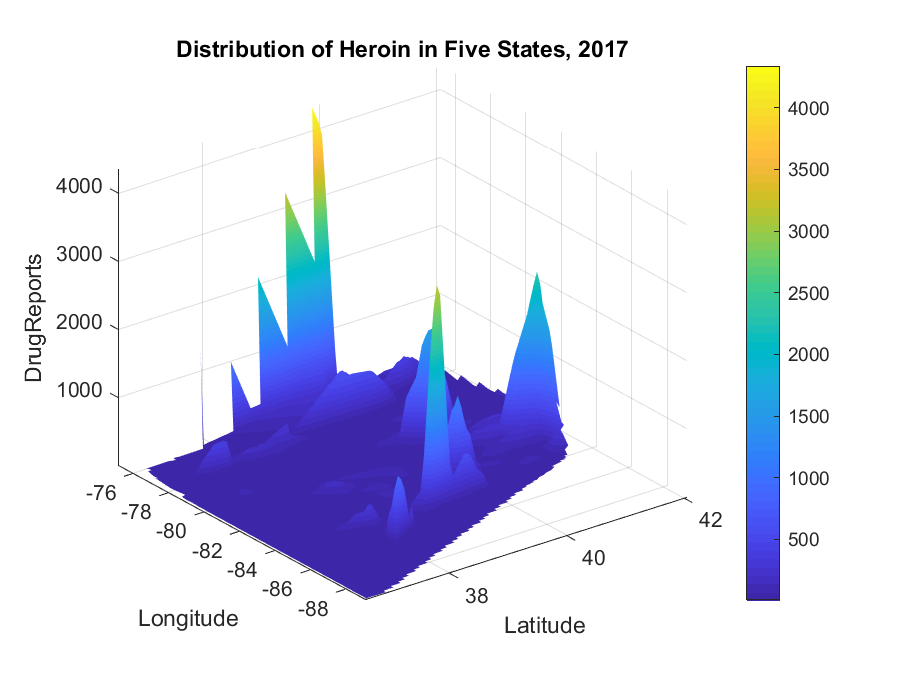
\includegraphics[width=0.7\textwidth]{./pictureb/Herion2017.eps}}
  \caption{Distribution of heroin cases in five states, 2017}\label{fighe17}
\end{figure}
%=============================================


 
% \begin{figure}
%\begin{minipage}[t]{0.5\linewidth}
%\centering
%\includegraphics[width=2.8in]{./picture/AZ.png}
%\caption{Energy profile for AZ}
%\label{fig:left:1}
%\end{minipage}%
%\begin{minipage}[t]{0.5\linewidth}
%\centering
%\includegraphics[width=2.9in]{./picture/CA.png}
%\caption{Energy profile for CA}
%\label{fig:right:1}
%\end{minipage}
%\end{figure}      

\subsection{ Spread Model Construction}

In order to describe the spread and characteristics of the reported synthetic opioid and heroin incidents in and between five states and their counties, we use the combination of two models to set up the spread model of opioids.

Firstly, we assume that the spread of opioids is like the diffusion of smoke during explosion, and derive a formula from {\bf{Smoke Diffusion Model}} that fits this problem\cite{b1}. Let the time when there is one case in a particular county be 0, denoted $t=0$. The position of this county is denoted as $(x_0,y_0)$, $x_0,\ y_0$ represent longitude and latitude, respectively. At time $t$, the number of cases in all five states is denoted as $Z(x,y,t)$. Analogous to the diffusion equation for smoke, we derive the following formula (\ref{eqsm}):
\begin{equation}
Z(x,y,t) = \frac{Q}{(kt)^{3/2}}\cdot \exp{\left[-\frac{(x-x_0)^2+(y-y_0)^2}{kt}\right]}
\label{eqsm}
\end{equation}
where $Q,\ k$ are two parameters determined by the practical data.

For more than one source, namely $n$ sources, we denote each starting location as $(x_{is},y_{is}), \ i=1,2,\cdots,n.$ For each source, the spread equation is:
\begin{equation}
Z_i(x,y,t) = \frac{Q_i}{(k_i\cdot t)^{3/2}}\cdot \exp{\left[-\frac{(x-x_{is})^2+(y-y_{is})^2}{k_i\cdot t}\right]},\quad i=1,2,\cdots,n.
\label{eqsmi}
\end{equation}
Therefore, the whole spread model of the opioids is explained by equation (\ref{eqwsm}):
\begin{equation}
\begin{aligned}
Z_w&=\sum\limits_{i=1}^n Z_i(x,y,t) \\
&=\sum\limits_{i=1}^n \frac{Q_i}{(k_i\cdot t)^{3/2}}\cdot \exp{\left[-\frac{(x-x_{is})^2+(y-y_{is})^2}{k_i\cdot t}\right]}.
\label{eqwsm}
\end{aligned}
\end{equation}

To calculate $Q_i$ and $k_i$ parameters, we first look at equation (\ref{eqsmi}). Take logarithm of both sides of the equation (\ref{eqsmi}), we get
\begin{equation}
\ln Z_i(x,y,t) = \ln Q_i - \frac{3}{2}\ln k_i\cdot t-\frac{(x-x_{is})^2+(y-y_{is})^2}{k_i\cdot t}.
\label{eqsmlog}
\end{equation}

We first find starting locations of every specific opioid. The method how to find resources will be explained in section (\ref{evm}). Substituting $x=x_{is}$ and $y=y_{is}$, we immediately get a relationship between $Q_i$ and $k_i$. Then we use points around the source to get auxiliary equations. Solving those equations, we can fit to get $Q_i$ and $k_i$ parameters and equations for every specific source.  Summing all the equations, we can obtain a whole model for demonstrating spread and characteristics of heroin and synthetic opioids cases in and between five states and their counties.

Secondly, Since the main problem need to be solved in Part1 is to describe the time-varying relationship between the propagation and characteristics of reported synthetic opioids and heroin events in various counties, time series is considered as another model to further analyze the location and future situation.

Considering the trend and periodicity of the data in the model, the third exponential smoothing model, {\bf{Holt-Winter exponential smoothing model}}, is used\cite{b2}.

The cubic exponential smoothing algorithm is based on the recursive relationship between the first and second exponential smoothing. The first exponential smoothing algorithm is based on the following recursive relationship:
\begin{equation}
s_i=\alpha\cdot x_i+(1-\alpha)\cdot s_{i-1}
\label{eqfirst}
\end{equation}
Where $\vec{s}$ is the smoothing value vector, $\vec{x}$ is data vector, number of cases in a particular county. The subscription $i$ represents the ith value of the vector. The equation (\ref{eqfirst}) shows that as $\alpha$ goes to 1, the smoothed value goes to the data value of the current time and the data is more uneven. And the closer $\alpha$ is to 0, the smoother the data is.

Quadratic exponential smoothing retains the trend information and adds a new variable to represent the trend after smoothing. The recurrence relationship is as follows:
\begin{equation}
\left\{
\begin{aligned}
s_i&=\alpha \cdot x_i+(1-\alpha)\cdot(s_{i-1}+t_{i-1})\\
t_i&=\beta\cdot(s_i-s_{i-1})+(1-\beta)\cdot t_{i-1}
\end{aligned}
\right.
\end{equation}
Where $\vec{t}$ is trend value vector.

The cubic exponential smoothing retains the periodic information on the basis of the quadratic exponential smoothing, which makes it possible to predict the time series with periodicity. The cumulative cubic exponential smoothing is used here.
\begin{equation}
\left\{
\begin{aligned}
s_i&=\alpha \cdot (x_i-p_{i-1})+(1-\alpha)\cdot(s_{i-1}+t_{i-1})\\
t_i&=\beta\cdot(s_i-s_{i-1})+(1-\beta)\cdot t_{i-1}\\
p_i&=\gamma\cdot(x_i-s_i)+(1-\gamma)\cdot p_{i-1}
\end{aligned}
\right.
\end{equation}
where $\vec{p}$ is periodic value vector; $\alpha,\ \beta, \ \gamma\in[0,1]$, and they are decided by the data provided, and can be adjusted according to practical situation. 

The prediction equation is:
\begin{equation}
x_{i+h}=s_i+h\cdot t_i+p_{i+h-1}, \quad h = 1,2,\cdots
%\label{eqfirst}
\end{equation}

Since the memory ability of exponential smoothing method is very short, the influence of initial value will become very weak. We assign the following initial value:
\begin{equation}
\left\{
\begin{aligned}
s_1&=x_1\\
t_1&=x_2-x_1\\
p_1&=0
\end{aligned}
\right.
\end{equation}
Then we can use the latitude, longitude and year corresponding to $\vec{x}$ to make up a matrix $X(x,y,t)=\vec{x}(t)$. Now since we have constructed two models, we combine them into one {\bf{Spread Model}} using equation (\ref{eqp1}) to get more accurate and convincing results.
\begin{equation}
Z_c=\frac{Z_w+X}{2}
\label{eqp1}
\end{equation}

\subsection{Spread and Characteristics}

Since plotting the number of reports of drugs with respect to latitude, longitude and time requires four dimensions, which is not able to bring an intuitive image of how opioids spread in and between the five states, we plot  the number of drug reports with respect to longitude and latitude separately, shown in figure (\ref{figl1}) to figure (\ref{figr2}).

 \begin{figure}[!htbp]
\begin{minipage}[t]{0.5\linewidth}
\centering
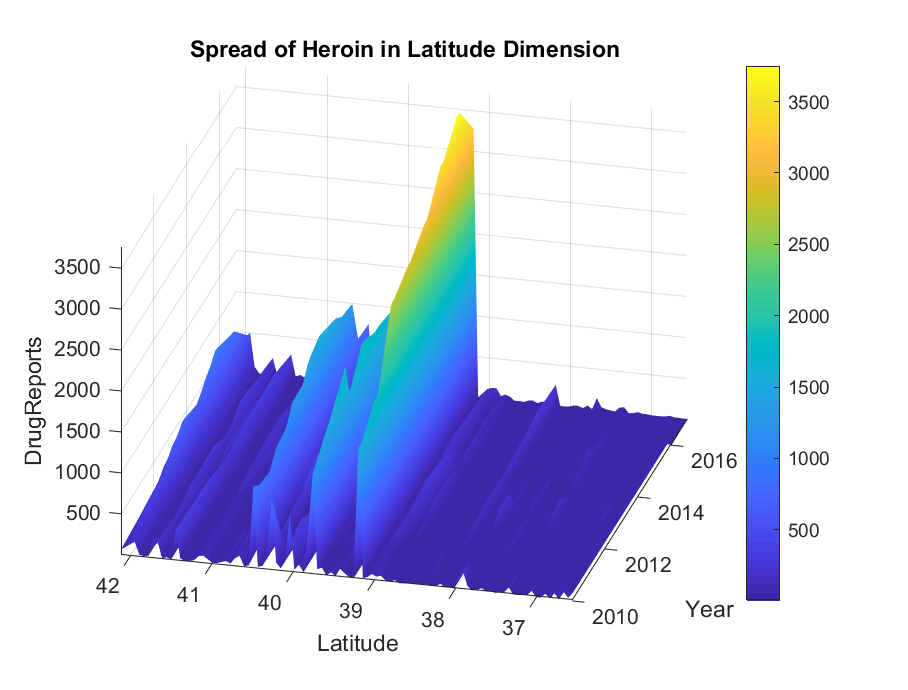
\includegraphics[width=2.8in]{./picture/sphela.eps}
\caption{Heroin Spread, Latitude}
\label{figl1}
\end{minipage}%
\begin{minipage}[t]{0.5\linewidth}
\centering
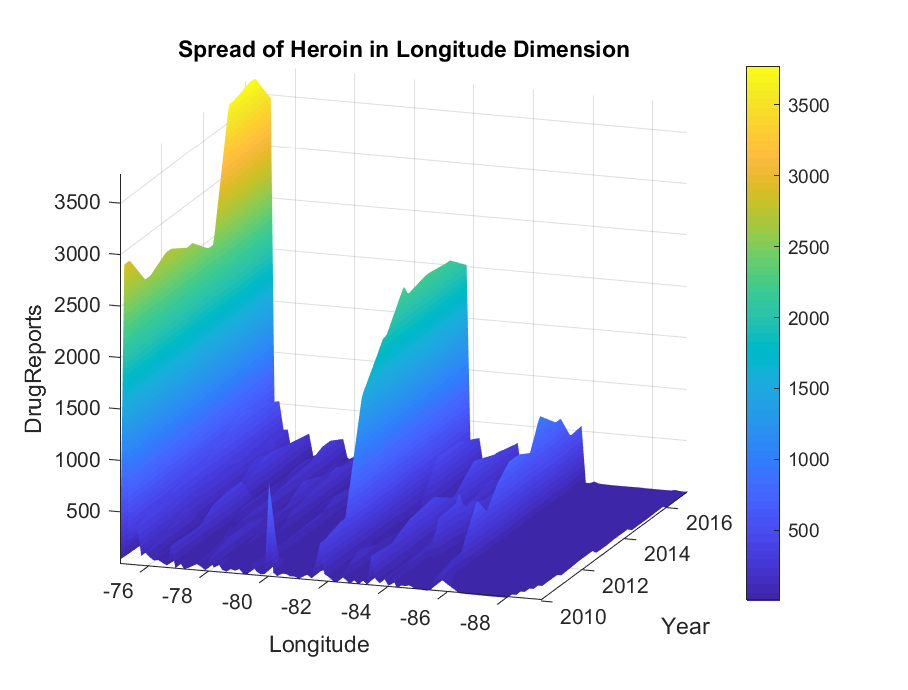
\includegraphics[width=2.8in]{./picture/sphelong.eps}
\caption{Heroin Spread, Longitude}
\label{figr1}
\end{minipage}
\end{figure}

 \begin{figure}[!htbp]
\begin{minipage}[t]{0.5\linewidth}
\centering
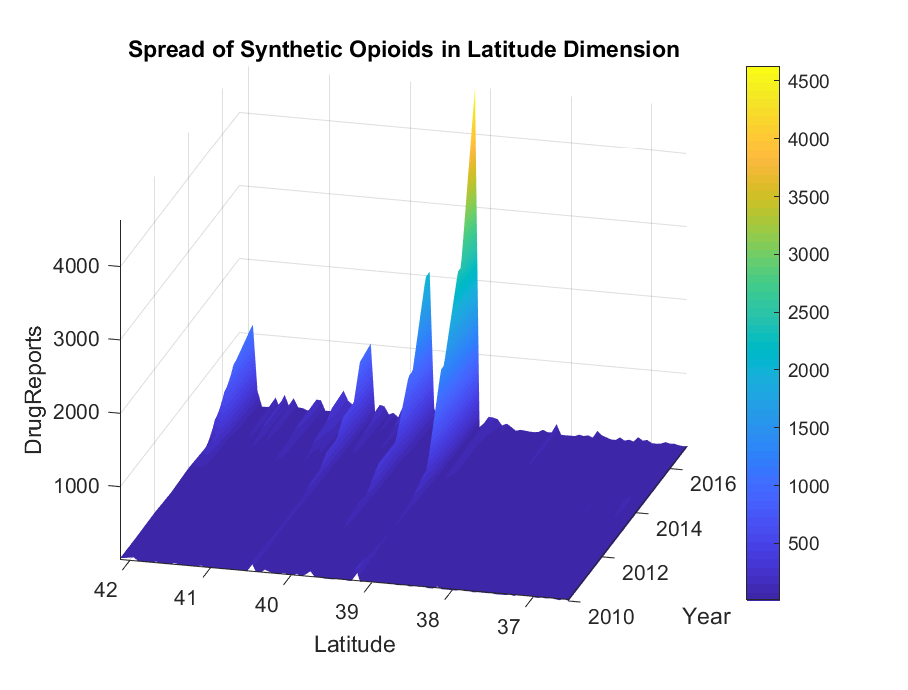
\includegraphics[width=2.8in]{./picture/spsola.eps}
\caption{Opioids Spread, Latitude}
\label{figl2}
\end{minipage}%
\begin{minipage}[t]{0.5\linewidth}
\centering
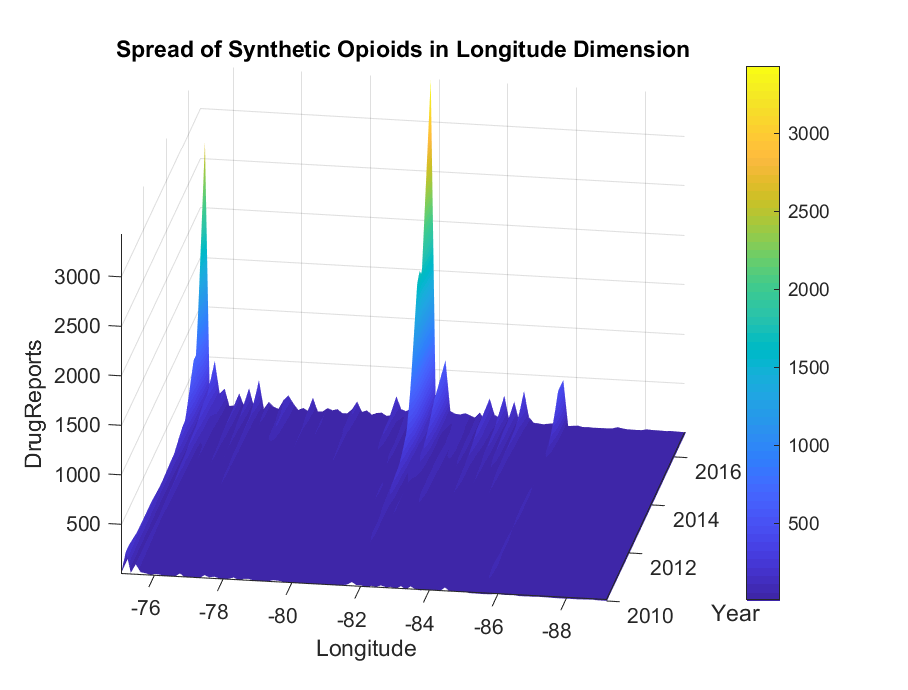
\includegraphics[width=2.8in]{./picture/spsolong.eps}
\caption{Opioids Spread, Longitude}
\label{figr2}
\end{minipage}
\end{figure}

Taking some counties as the center, it gradually spread outward to more counties. At the beginning, there are more heroin reports in some counties (more than 100 cases). Then it is found that the number of heroin reports in neighboring counties will increase year by year, and the situation of synthetic opioids is similar: some counties start drug abuse earlier and neighbors are very likely to follow.

We can see that in general the number of heroin cases increase from 2010 to 2017, however, if we look at certain counties, the number of heroin cases decrease  2017. But for synthetic opioids, most of them increase dramatically from 2016 to 2017. For both heroin and synthetic opioids, there are only several counties that have tremendous quantities of cases, and most counties possess a relatively small amount of cases. {\bf{Cuyahoga (OH), Hamilton (OH), Allegheny (PA) and Philadelphia (PA)}} are four counties that almost have the largest number of both heroin cases and synthetic opioids cases, while  {\bf{Montgomery (OH)}} counties has a great amount of synthetic opioids cases but the heroin cases are relatively less. And we can also know that {\bf {Ohio and Pennsylvania}} are two states that drug abuse situations are the most serious.

\subsection{Identify Starting Locations}
\label{evm}

We construct a  {\bf{Extreme Value Model}} to find the starting locations\cite{b3}. Let $Z$ be the number of cases of heroin or synthetic opioids, $Z = Z(x,y)$ is a function of $x,\ y$ at a specific year. $x,\ y$ are latitude and longitude of each county respectively. We see $Z(x_i,y_i)$ as a source if it satisfies the following equation (\ref{eqcon}):
\begin{equation}
\left\{
\begin{aligned}
Z(x_i,y_i)&\geqslant Z(x_{i},y_{i+1})\\
Z(x_i,y_i)&\geqslant Z(x_{i},y_{i-1})\\
Z(x_i,y_i)&\geqslant Z(x_{i+1},y_{i})\\
Z(x_i,y_i)&\geqslant Z(x_{i-1},y_{i})\\
Z(x_i,y_i)&\geqslant Z(x_{i+1},y_{i+1})\\
Z(x_i,y_i)&\geqslant Z(x_{i-1},y_{i+1})\\
Z(x_i,y_i)&\geqslant Z(x_{i+1},y_{i-1})\\
Z(x_i,y_i)&\geqslant Z(x_{i-1},y_{i-1})\\
\end{aligned}
\right.
\label{eqcon}
\end{equation}

We use this method to find sources $(x_i,y_i)$ year by year for a specific opioid, and integration all the sources found in one or more years, making up a set $\{X,Y\}$ that contains all the possible starting locations.

The starting locations of heroin and synthetic opioids are shown in figure (\ref{fig:left:1}) and (\ref{fig:right:1}), respectively.

 \begin{figure}[!htbp]
\begin{minipage}[t]{0.5\linewidth}
\centering
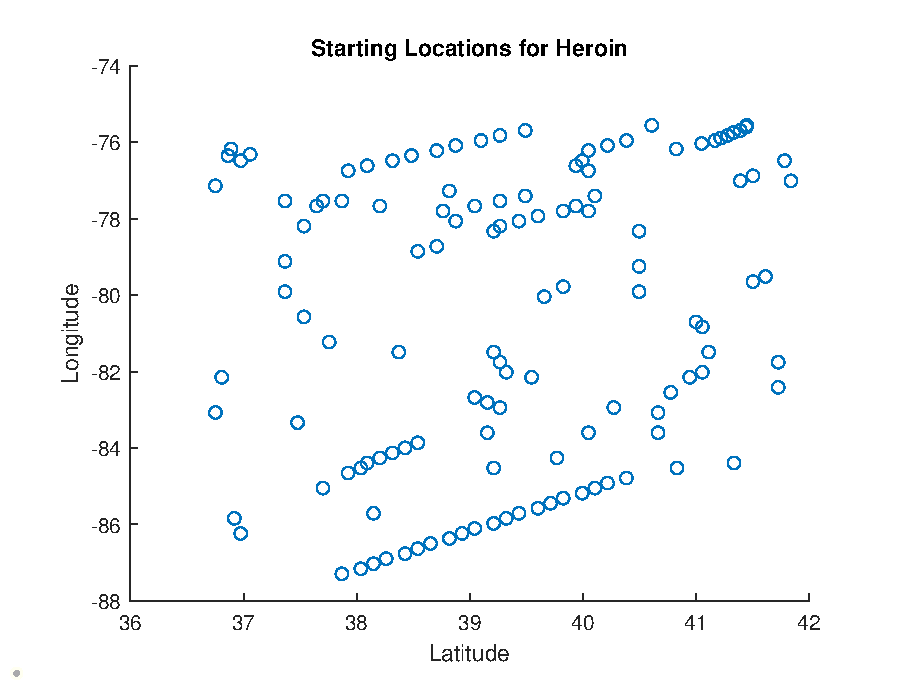
\includegraphics[width=2.8in]{./picture/startlocationhe.eps}
\caption{Sources of Heroin}
\label{fig:left:1}
\end{minipage}%
\begin{minipage}[t]{0.5\linewidth}
\centering
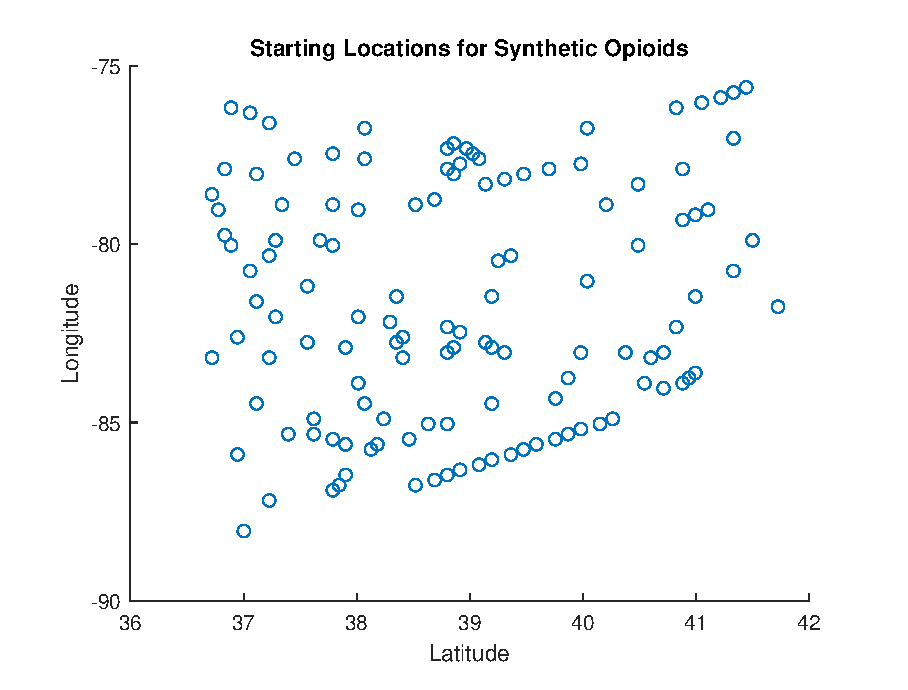
\includegraphics[width=2.8in]{./picture/startlocationso.eps}
\caption{Sources of Opioids}
\label{fig:right:1}
\end{minipage}
\end{figure} 


\subsection{Prediction}

\subsubsection{Government Concerns}

Observing the trends of drug reports in figure (\ref{figl1}) to figure (\ref{figr2}), we find that there exist many counties that the number of drug reports are increasing year by year and there are even some counties that the number increasing dramatically during recent years. Besides, there are some counties that the number of reports are too large that exceed several thousand. In the meantime, there are also many counties that just begin to have drug reports.

By the analysis above, we put forward three concerns for U.S. government to pay attention to:
\begin{enumerate}
\item For counties that only begin to abuse drugs, we should kill this phenomenon in the cradle;
\item  For counties that the number of drug reports increase rapidly, we should limit their acceleration and do not let them goes too swiftly;
\item For counties that already have a great number of drug reports, we should isolate them and do not let them spread drugs to other counties.
\end{enumerate}

\subsubsection{Threshold Levels}

Corresponding to the three concerns above, we set three threshold levels:
\begin{enumerate}
\item {\bf{Critical threshold level}}: the threshold whether one county begins to abuse drugs;
\item {\bf{Alarm threshold level}}: the threshold whether one county gets to the fastest increasing speed;
\item {\bf{Diffusion threshold level}}: the threshold whether one county arrives at its peak number of drug reports.
\end{enumerate}

We use equation (\ref{eqsm}) to calculate the three threshold levels. We first find out the {\bf{diffusion threshold level}}. The condition is that the increasing speed is zero. Let the derivative of equation (\ref{eqsm}) over $t$ be zero, we get
\begin{equation}
\begin{aligned}
&{\frac{\partial Z}{\partial t}}
={\frac {\partial }{\partial t}} \left[ {\frac {Q}{ \left( kt \right) ^
{3/2}}{{\rm e}{-{\frac { \left( x-x_0 \right) ^{2}+ \left( y-y_0 \right) 
^{2}}{kt}}}}} \right] \\
&=-{\frac {3Qk}{2 \left( kt \right) ^{5/2}}{
{\rm e}^{-{\frac { \left( x-x_0 \right) ^{2}+ \left( y-y_0 \right) ^{2}}{k
t}}}}}+{\frac {Q \left[  \left( x-x_0 \right) ^{2}+ \left( y-y_0 \right) ^
{2} \right] }{ \left( kt \right) ^{3/2}k{t}^{2}}{{\rm e}^{-{\frac {
 \left( x-x_0 \right) ^{2}+ \left( y-y_0 \right) ^{2}}{kt}}}}}\\
 &=0
\end{aligned}
\label{eqder}
\end{equation}
Solving equation (\ref{eqder}), we get
\begin{equation}
t_1=\frac{2}{3}\cdot\frac{(x-x_0)^2+(y-y_0)^2}{k}
\end{equation}

Then we decide the {\bf{alarm threshold level}}. calculate the second derivative of equation (\ref{eqsm}):
\begin{equation}
\begin{aligned}
&{\frac {\partial ^{2}}{\partial {t}^{2}}} \left[ {\frac {Q}{ \left( kt
 \right) ^{3/2}}{{\rm e}^{-{\frac { \left( x-x_0 \right) ^{2}+ \left( y-
y_0 \right) ^{2}}{kt}}}}} \right] \\
&={\frac {15\,Q{k}^{2}}{4\, \left( kt
 \right) ^{7/2}}{{\rm e}^{-{\frac { \left( x-x_0 \right) ^{2}+ \left( y-
y_0 \right) ^{2}}{kt}}}}}\\
&\quad-3\,{\frac {Q \left[  \left( x-x_0 \right) ^{2}+
 \left( y-y_0 \right) ^{2} \right] }{ \left( kt \right) ^{5/2}{t}^{2}}{
{\rm e}^{-{\frac { \left( x-x_0 \right) ^{2}+ \left( y-y_0 \right) ^{2}}{k
t}}}}}\\
&\quad-2\,{\frac {Q \left[  \left( x-x_0 \right) ^{2}+ \left( y-y_0
 \right) ^{2} \right] }{ \left( kt \right) ^{3/2}k{t}^{3}}{{\rm e}^{-{
\frac { \left( x-x_0 \right) ^{2}+ \left( y-y_0 \right) ^{2}}{kt}}}}}\\
&\quad+{
\frac {Q \left[  \left( x-x_0\right) ^{2}+ \left( y-y_0 \right) ^{2}
 \right] ^{2}}{ \left( kt \right) ^{3/2}{k}^{2}{t}^{4}}{{\rm e}^{-{
\frac { \left( x-x_0\right) ^{2}+ \left( y-y_0 \right) ^{2}}{kt}}}}}
\end{aligned}
\label{eqdre2}
\end{equation}
Let equation (\ref{eqdre2}) be zero, we get
\begin{equation}
t_2=2\cdot\left(\frac{1}{3}\pm\frac{1}{15}\right)\cdot\frac{(x-x_0)^2+
(y-y_0)^2}{k}
\end{equation}

The time $t$ first arrives at smaller value, thus the bigger value is unrealistic. Adopt minus sign, we get

\begin{equation}
t_2=\frac{8}{15}\cdot\frac{(x-x_0)^2+(y-y_0)^2}{k}
\end{equation}

Finally, we figure out the {\bf{critical threshold level}}. Here in our models, $Z$  from 0 to 1 means that one county begin to abuse opioids. Let $Z=1$ in equation (\ref{eqsm}), we get
\begin{equation}
0= \ln Q - \frac{3}{2}\ln k\cdot t-\frac{(x-x_{0})^2+(y-y_{0})^2}{k\cdot t}.
\end{equation}
Solving this equation, we get
\begin{equation}
t_3 = \frac{k\ln Q\pm\sqrt{\Delta}}{3k\ln k}, 
\end{equation}
where
\begin{equation}
\Delta=(k\ln Q)^2-6k\ln k\cdot
\left[(x-x_{0})^2+(y-y_{0})^2\right].
\end{equation}

Here we should choose the smaller $t_3$, thus using minus sign.
\begin{equation}
t_3 = \frac{k\ln Q-\sqrt{\Delta}}{3k\ln k}, 
\end{equation}

The threshold levels are 
\begin{equation}
\left\{
\begin{aligned}
Z &= Z(x,y,t_1),\ \text{diffusion threshold level},\\
Z&=Z(x,y,t_2),\ \text{alarm threshold level},\\
Z&=Z(x,y,t_3),\ \text{critical threshold level},
\end{aligned}
\right.
\label{eqZ}
\end{equation}
where
\begin{equation}
\left\{
\begin{aligned}
t_1&=\frac{2}{3}\cdot\frac{(x-x_0)^2+(y-y_0)^2}{k},\\
t_2&=\frac{8}{15}\cdot\frac{(x-x_0)^2+(y-y_0)^2}{k},\\
t_3 &= \frac{k\ln Q-\sqrt{\Delta}}{3k\ln k}.
\end{aligned}
\right.
\label{eqt}
\end{equation}

Then for every county, we substitute longitude and latitude into equation (\ref{eqt}) to get the time $t_i,\ i=1,\ 2,\ 3$. Substituting $x,\ y,\ t_i$ into equation (\ref{eqZ}), we obtain the threshold levels, respectively. For example, the alarm threshold levels of heroin and synthetic opioids are shown in figure (\ref{fig:left:3}) and figure (\ref{fig:right:3}).

 \begin{figure}[!htbp]
\begin{minipage}[t]{0.5\linewidth}
\centering
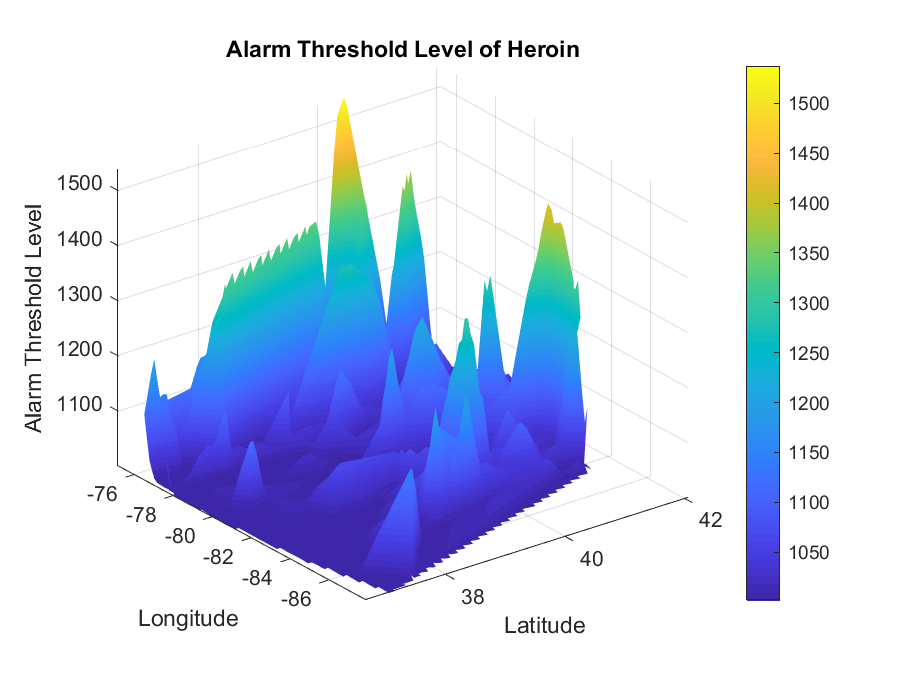
\includegraphics[width=2.8in]{./picture/athe.eps}
\caption{Alarm Threshold, Heroin}
\label{fig:left:3}
\end{minipage}%
\begin{minipage}[t]{0.5\linewidth}
\centering
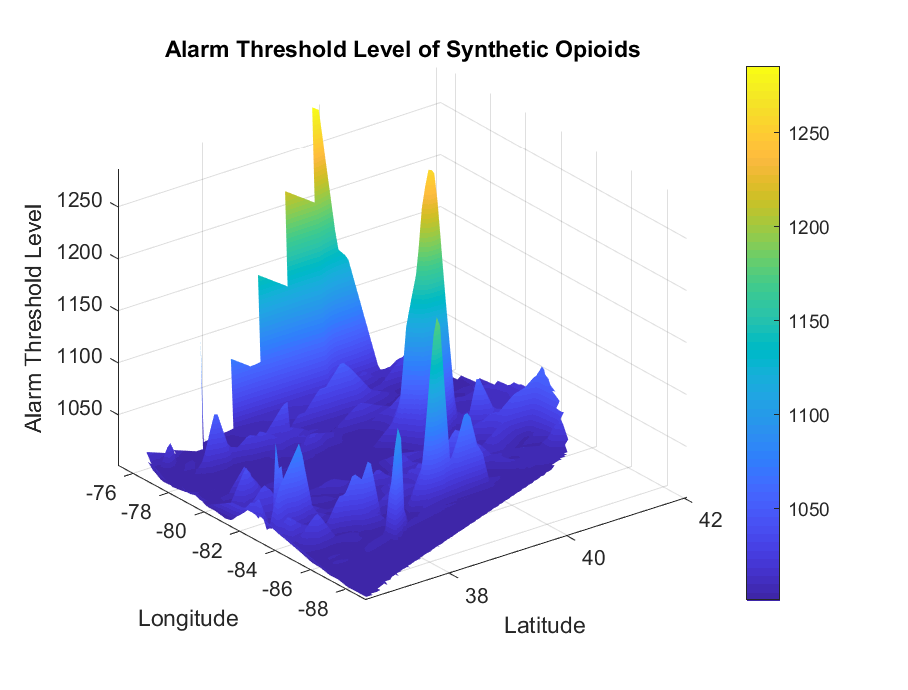
\includegraphics[width=2.8in]{./picture/atso.eps}
\caption{Alarm Threshold, Opioids}
\label{fig:right:3}
\end{minipage}
\end{figure} 

\subsubsection{Places and Time}

Using equation (\ref{eqZ}), equation (\ref{eqt}) and equation (\ref{eqp1}), we are able to obtain the time and places of all specific opioids for diffusion threshold level, alarm threshold level and critical threshold level. For example, the time and places of heroin and synthetic opioids cases for alarm threshold level are shown in figure (\ref{fig:left:4}) and figure (\ref{fig:right:4}).

\begin{figure}[!htbp]
\begin{minipage}[t]{0.5\linewidth}
\centering
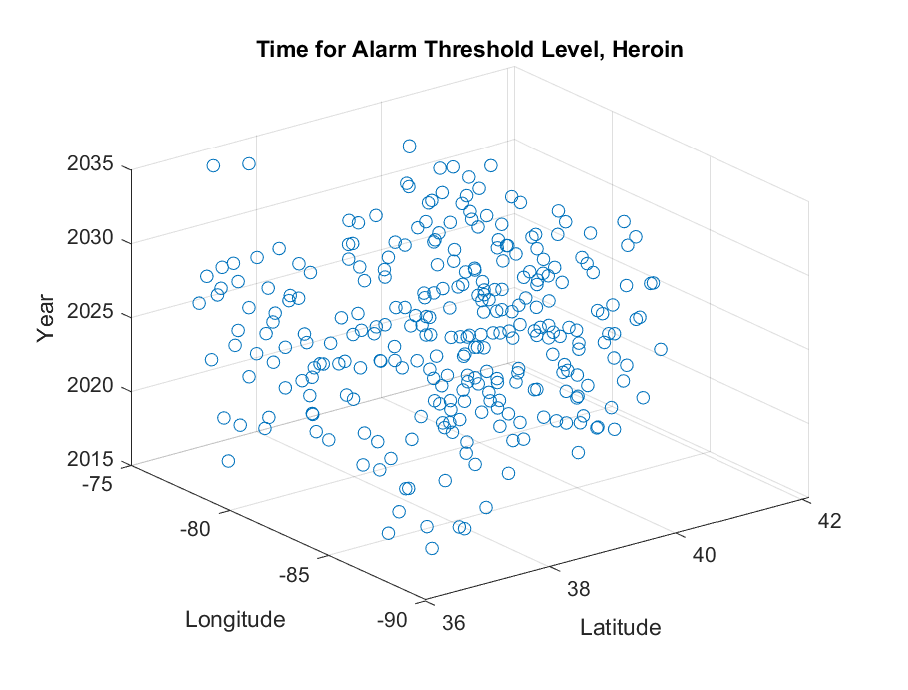
\includegraphics[width=2.8in]{./picture/timehe.eps}
\caption{Time and Places, Heroin}
\label{fig:left:4}
\end{minipage}%
\begin{minipage}[t]{0.5\linewidth}
\centering
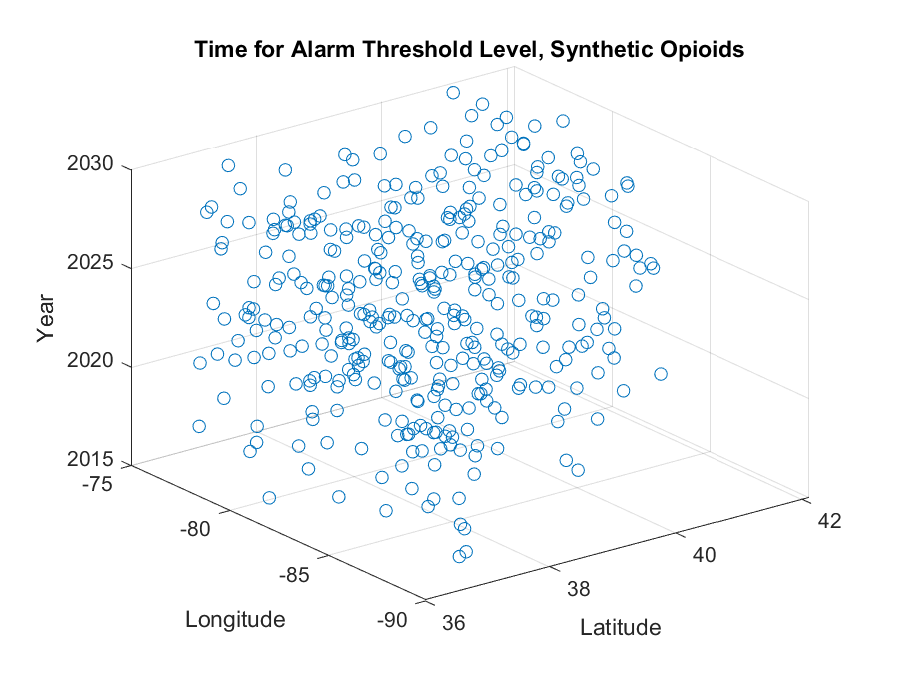
\includegraphics[width=2.8in]{./picture/timeso.eps}
\caption{Time and Places, Opioids}
\label{fig:right:4}
\end{minipage}
\end{figure} 



\section{Part 2}

\subsection{Initial Data Analysis}

In the data set provided for part 2, there are some percentage data have some error of input, we delete them all.

\subsection{Model Construction}

Firstly, the type of the data is long panel, since the number of states $n$ is less than the number of years $T$. In order to control individual effects, generate the dummy variables of state\cite{b5}:
\begin{equation}
\text{State 2}=
\left\{
\begin{aligned}
&1,\ \text{State OH; }\\
&0,\ \text{State KY}
\end{aligned}
\right.
\end{equation}
\begin{equation}
\text{State 3}=
\left\{
\begin{aligned}
&1,\ \text{State PA; }\\
&0,\ \text{State KY}
\end{aligned}
\right.
\end{equation}
\begin{equation}
\text{State 4}=
\left\{
\begin{aligned}
&1,\ \text{State VA; }\\
&0,\ \text{State KY}
\end{aligned}
\right.
\end{equation}
\begin{equation}
\text{State 5}=
\left\{
\begin{aligned}
&1,\ \text{State WV; }\\
&0,\ \text{State KY}
\end{aligned}
\right.
\end{equation}

Secondly, $T$ is a only little bigger than $n$, so $T$ can not provide enough information to estimate autoregressive coefficient of every panel, so we assume they are all equal\cite{b6}. Use time trend variable $t$ to consider about the time effect.

Thirdly, we choose variables. The provided U.S. Census Bureau socio-economic data has a lot of variables which makes analysis of these data sophisticated. Observing all the variables, we find that every four columns data refers to one variable except for the first three variables. Then we subtract one fourth data of different variables to analyze. By the meaning of each variable, we divide all variables into 16 categories, shown in table (\ref{tab:p2i}).

\vspace{-0.3cm}
\begin{table}[htbp]
  \centering
  \caption{Variable Categories in U.S. Census Bureau Data}
    \begin{tabular}{cl}
    \addlinespace
    \toprule[1.5pt]
    Number & Variable Categories \\
    \midrule[1pt]
        1     & Geography \\
    2     & Households by type \\
    3     & Relationship \\
    4     & Marital status \\
    5     & Fertility \\
    6     & Grandparents \\
    7     & School enrollment \\
    8     & Educational attainment \\
    9     & Veteran status \\
    10    & Disability status of the civilian non institutionalized population \\
    11    & Residence 1 year ago \\
    12    & Place of birth \\
    13    & U.S. citizenship status \\
    14    & Year of entry \\
    15    & World region of birth of foreign born \\
    16    & Language spoken at home \\
    17    & Ancestry \\
    \bottomrule[1.5pt]
    \end{tabular}%
  \label{tab:p2i}%
\end{table}%

In addition, the variables also include point estimate, percent estimate, the standard error of point estimate and the standard error of percent estimate.
There are so many variables, so we use three steps to screen variables, the steps are as follows.

\begin{enumerate}
\item The model of estimating two-way fixed effects using LSDV\cite{b7}

Consider all the data of economic and social census into regression as variables. It's a fixed effect model not a stochastic effect model, since we consider the dummy variables. Omit variables which have obvious multicollinearity or have very small regression estimation parameters.
We use clustering robustness standard coefficient (considering autocorrelation of different disturbance terms of the same state), but there are too many variables, we can't calculate $t$ value and $p$ value.
\item Stepwise Regression

Using Stepwise Regression carrying out surplus variables,the backward elimination procedure begins with a model that includes all the independent variables. It then deletes one independent variable at a time using the same procedure as stepwise regression. Set AIpha = 0.05.
\item Best-Subsets Regression\cite{b8}

Using Best-Subsets Regression to carry out remain variables. Consider both reducing variables and making R-Sq bigger to get final variables.
\end{enumerate}

Fourthly, we test long panel data about heteroscedasticity and autocorrelation:
\begin{enumerate}[]
\item Test of heteroscedasticity between groups

We first make an assumption: $H_0:\ \sigma_i^2=\sigma^2,\ i=1,2,\cdots,n.$
Using Wald test\cite{b9}, the result strongly rejects the assumption of homogeneity between groups, illustrating that different states have different situations.
\item Intra group autocorrelation

Under the original assumption that there do not exist intra group autocorrelation, the variance and autocovariance of the disturbance term $\Delta\epsilon_{it}$ are:
\begin{equation}
Var(\Delta\epsilon_{it})=Var(\epsilon_{it}-\epsilon_{i,t-1})
=Var(\epsilon_{it}) + Var(\epsilon_{i,t-1}) = 2\sigma_\epsilon^2
\end{equation}
\begin{equation}
\begin{aligned}
Cov(\Delta\epsilon_{it},\Delta\epsilon_{i,t-1})
&=Cov(\epsilon_{it}-\epsilon_{i,t-1},\epsilon_{i,t-1}-\epsilon_{i,t-2})\\
&=-Cov(\epsilon_{i,t-1},\epsilon_{i,t-1})\\
&=-Var(\epsilon_{i,t-1})=-\sigma_\epsilon^2
\end{aligned}
\end{equation}
Then the autocorrelation coefficient is:
\begin{equation}
Corr(\Delta\epsilon_{it},\Delta\epsilon_{i,t-1})
=\frac{Cov(\Delta\epsilon_{it},\Delta\epsilon_{i,t-1})}
{Var(\Delta\epsilon_{it})}
=\frac{-\sigma_\epsilon^2}{2\sigma_\epsilon^2}
=-0.5
\end{equation}
Denote the sample value of $\Delta\epsilon_{it}$ as $e_{it}$, then carry out first order autoregression upon $e_{it}$:
\begin{equation}
e_{it}=\rho e_{i,t-1}+error_{it}, \ i=1,\cdots,n;\ t=3,\cdots,T.
\end{equation}
Then we perform Wald test upon ``$H_0:\ \rho=-0.5$''. The results strongly reject the original hypothesis that there is no first order intra group autocorrelation.
\item Cross sectional correlation test

Consider the original hypothesis ``there is no component cross-section correlation''. If this hypothesis holds, then the correlation coefficients between individual perturbation terms calculated by residual error should be close to zero. If we arrange there correlation coefficients to a matrix, that is, correlation matrix of residuals, then the non-principal diagonal elements are close to 0.

With insufficient evidence to reject $H_0$, considering the second error is enough small, we accept $H_0$, illustrating individual disturbance terms are independent, indicating that the disturbance factors of drug use in different states are exogenous and almost unrelated.
\end{enumerate}

Fifthly, we carry out regression. we deal with Intra group autocorrelation's and group synchronization's FGLS at the same time. We find that different individual disturbance terms are relevant but have different variance. There are some autocorrelations having the same autocorrelation coefficients in the same group.

\subsection{Model Results}
The significant variables for synthetic opoids are shown in table (\ref{tab:sov}).

% Table generated by Excel2LaTeX from sheet 'Sheet1'
\begin{table}[htbp]
  \centering
  \caption{Significant Variables for Synthetic Opoids Cases}
    \begin{tabular}{cl}
    \addlinespace
    \toprule[1.5pt]
    Number & Variables \\
    \midrule[1pt]
    
    1     & Estimate; HOUSEHOLDS BY TYPE - Nonfamily households\\
    & - Householder living alone - 65 years and over \\
    2     & Estimate; RESIDENCE 1 YEAR AGO - Abroad \\
    3     & Estimate; GRANDPARENTS - Who are married \\
    4     & Estimate; SCHOOL ENROLLMENT - College or graduate school \\
    5     & Estimate; EDUCATIONAL ATTAINMENT - 9th to 12th grade, \\
    &no diploma \\
    6     & Estimate; EDUCATIONAL ATTAINMENT - Associate's degree \\
    7     & Estimate; EDUCATIONAL ATTAINMENT - Percent high \\
    & school graduate or higher \\
    8     & Estimate; LANGUAGE SPOKEN AT HOME - Language other \\
    &than English - Speak English less than "very well" \\

    \bottomrule[1.5pt]
    \end{tabular}%
  \label{tab:sov}%
\end{table}%

Then we use the upper limits and the lower limits $E_u,\ E_l, \ P_u,\ P_l$ to repeat the above steps. We find that the results are relevant. Since the  standard error/estimate is small, we ignore it.

For heroin cases, we perform the same procedures as synthetic opioids. The significant variables for heroin cases are shown in table (\ref{tab:she}).

% Table generated by Excel2LaTeX from sheet 'Sheet1'
\begin{table}[htbp]
  \centering
  \caption{Significant Variables for Heroin Cases}
    \begin{tabular}{cl}
    \addlinespace
    \toprule[1.5pt]
    Number & Variables \\
    \midrule[1pt]
    1     & Estimate; ANCESTRY – German \\
    2     & Estimate; DISABILITY STATUS OF THE CIVILIAN NON\\ & INSTITUTIONALIZED  POPULATION - With a disability \\
    3     & Estimate; FERTILITY - Number of women 15 to 50 years old who\\
    & had a birth in the past 12 months \\
    4     & Estimate; HOUSEHOLDS BY TYPE - Households with one or \\
    &more people 65 years and over \\
    5     & Estimate; VETERAN STATUS - Civilian veterans \\
    6     & Estimate; RELATIONSHIP - Other relatives \\
    \bottomrule[1.5pt]
    \end{tabular}%
  \label{tab:she}%
\end{table}%

Since the order of magnitude between other variables and dummy variables is large, resulting that the coefficients of dummy variables are large,so we consider using the percent estimate.




\subsection{Modify Model in Part 1}

Firstly, we use {\bf{Principal Components Analysis (PCA)}} to get a modified parameter $\alpha$ for the first model built in part 1.

\begin{enumerate}[]
\item
The main explanatory variables obtained by regression are analyzed by principal component factor analysis, and the factors whose eigenvalue are less than 1 are removed.
\item
Since the factors are correlated, the factors are rotated obliquely.
\item
Using factor scores to standardize each variable to have a zero mean and variance equals to 1. Perform weighted summation upon factor scores coefficients, formating linear composites.
\item
Calculate each factor and use combination weighting approach to get the coefficient $\alpha_i$ for each state at a specific year.
\end{enumerate}

Then we get the first modified spread model:
\begin{equation}
\begin{aligned}
Z_{wm}&=\sum\limits_{i=1}^n (1+\alpha_i)\cdot Z_i(x,y,t) \\
&=\sum\limits_{i=1}^n (1+\alpha_i)\cdot\frac{Q_i}{(k_i\cdot t)^{3/2}}\cdot \exp{\left[-\frac{(x-x_{is})^2+(y-y_{is})^2}{k_i\cdot t}\right]}.
\label{eqwsmm}
\end{aligned}
\end{equation}

Secondly, we modify the second model built in part 1. We have known from part 2 that the influence factors of synthetic opioids and their correlation coefficients $w_j, \ j=1,2,\cdot,n$, $n$ is the total number of correlation coefficients. We have known from the model of part 1 that the assumption is that the factors that influence the development of objective things in the past and at present also determine the development of future things. In other words, when these influence factors change, it will influence the direction of the whole model. According to the model of part 2, we simplify this question and assume that  these changes only influence the value of the trend vector, so the second modified model is as following:
\begin{equation}
\left\{
\begin{aligned}
s_i&=\alpha \cdot (x_i-p_{i-1})+(1-\alpha)\cdot(s_{i-1}+t_{i-1})\\
t_i&=\beta\cdot(s_i-s_{i-1})+(1-\beta)\cdot t_{i-1}\\
p_i&=\gamma\cdot(x_i-s_i)+(1-\gamma)\cdot p_{i-1}+
\sum\limits_{j=1}^n w_j\Delta m_j\\
x_{i+h}&=s_i+h\cdot t_i+p_{i+h-1}, \quad h = 1,2,\cdots
\end{aligned}
\right.
\end{equation}
Where $w_j$ means the correlation coefficients of the $j^{th}$ influence factor, and $\Delta m_j$ means the variation of $j^{th}$ influence factor. 

Then we can use the latitude, longitude and year corresponding to $\vec{x}$ to make up a modified matrix $X_m(x,y,t)=\vec{x}(t)$. Now since we have constructed two modified models, we combine them into one {\bf{Modified Spread Model}} using equation (\ref{eqpm}) to get more accurate and convincing results.
\begin{equation}
Z_{cm}=\frac{Z_{wm}+X_m}{2}
\label{eqpm}
\end{equation}

\section{Part 3}

\subsection{Identify A Possible Strategy}

According to part 2, we have known that there are many factors that will influence the values. Among them there are more factors are concerning about education. Therefore we set the following strategy: Improve the {\bf{education}} level of these five states, make sure that all the students (even adults) accept high school education (if accepted, college education), and popularize the knowledge of synthetic opioids and heroin.

\subsection{Effectiveness Test and Significant Parameter Bounds}

In the section, we use the number of drug reports as the significant parameter. And we think that when the drug reports number of five states in a year reduce 2\% comparing with that without the strategy, we success. That is to say, we set the significant parameter bounds to be 2\%. When the strategy becomes effective, it will influence the following four factors:
\begin{itemize}[]
\item Estimate; SCHOOL ENROLLMENT - College or graduate school;
\item Estimate; EDUCATIONAL ATTAINMENT - 9th to 12th grade;
\item
Estimate; EDUCATIONAL ATTAINMENT - Associate's degree;
\item  Estimate; EDUCATIONAL ATTAINMENT - Percent high school graduate or higher.
\end{itemize}

Assume that the four factors change similarly, we can get the following figure (\ref{figpre18}) to figure (\ref{figpre20}).

%=====图片格式:eps或者pdf=========================
\begin{figure}[!htbp]
  \centering{
  \includegraphics[width=0.55\textwidth]{./picturec/2018pre.eps}}
  \caption{Drug Reports' Reducing Percentage, 2018}\label{figpre18}
\end{figure}
%=============================================
%=====图片格式:eps或者pdf=========================
\begin{figure}[!htbp]
  \centering{
  \includegraphics[width=0.55\textwidth]{./picturec/2019pre.eps}}
  \caption{Drug Reports' Reducing Percentage, 2019}\label{figpre19}
\end{figure}
%=============================================
%=====图片格式:eps或者pdf=========================
\begin{figure}[!htbp]
  \centering{
  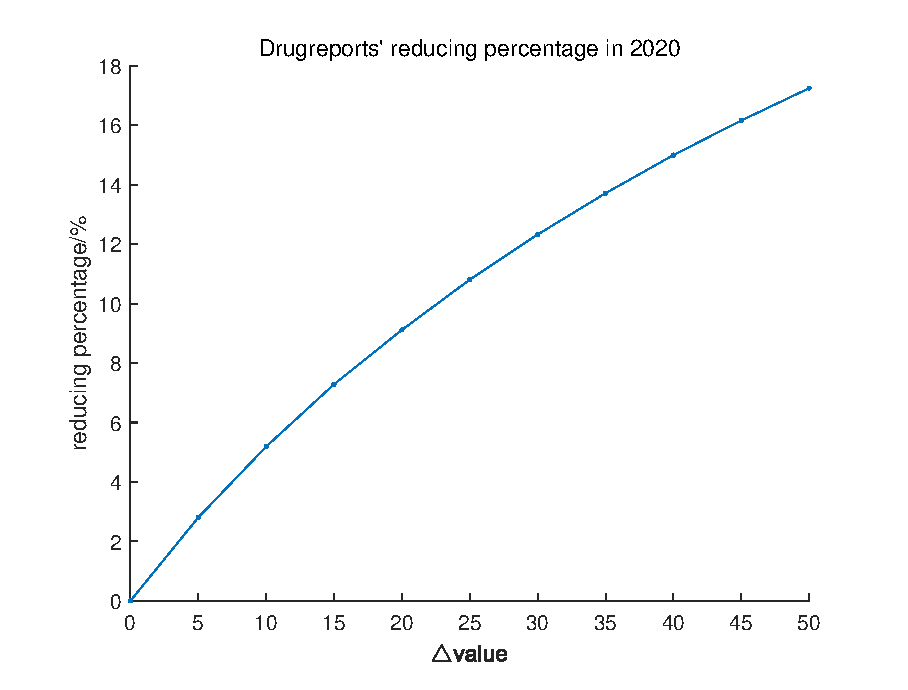
\includegraphics[width=0.55\textwidth]{./picturec/2020pre.eps}}
  \caption{Drug Reports' Reducing Percentage, 2020}\label{figpre20}
\end{figure}
%=============================================
%\begin{figure}[!htbp]
%\begin{minipage}[t]{0.5\linewidth}
%\centering
%\includegraphics[width=2.8in]{./picturec/2019pre.eps}
%\caption{Reducing Percentage, 2019}
%\label{figpre19}
%\end{minipage}%
%\begin{minipage}[t]{0.5\linewidth}
%\centering
%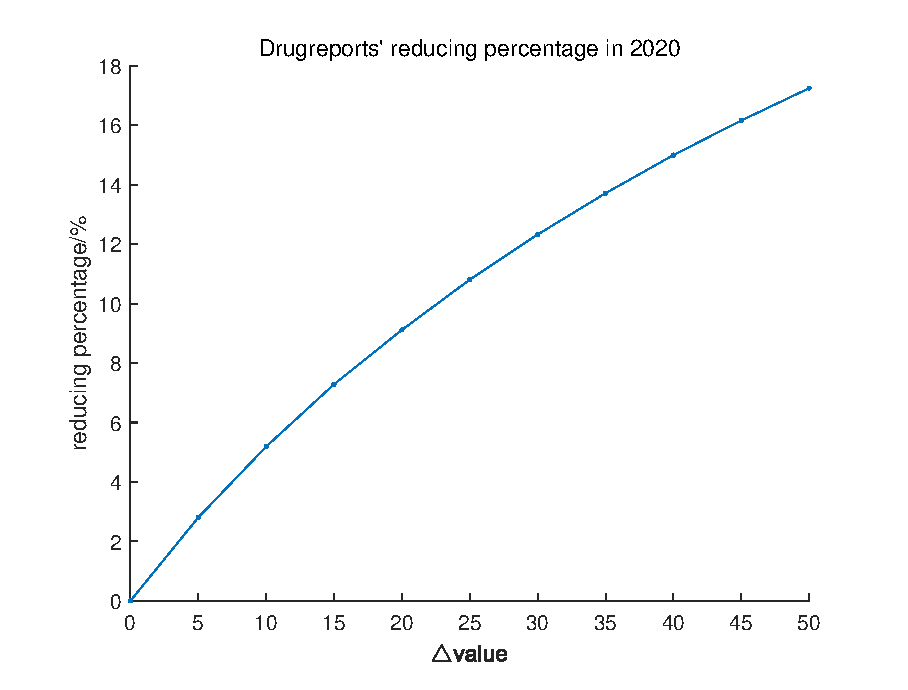
\includegraphics[width=2.8in]{./picturec/2020pre.eps}
%\caption{Reducing Percentage, 2020}
%\label{figpre20}
%\end{minipage}
%\end{figure} 

The X-axis represents the sum of changing values of these four factors, and the Y-axis represents the reducing percentage of the drug reports compared with that without the strategy. It's obvious that as time goes on, the reducing percentages are bigger, thus the influence degree is increasing. In 2018, when the changing values exceed 15, the percentage exceed 2\%. In 2019, the critical value is 10 and in 2020 the value is 5. Therefore, according to the judgment basis, this strategy successes.


\section{Evaluation of Models}

\subsection{Strengths}

\begin{itemize}
  \item We perform {\bf{initial data processing}}, add {\bf{longitude and latitude data}} to every county, categorize data into different types, which are beneficial for successive analysis and results display;
  \item We construct the {\bf{Spread Model}} with two different models, which is more accurate and convincing;
  \item We use {\bf{Extreme Value Model }} to find the starting locations of cases, which is convenient and easy to perform;
  \item We put forward {\bf{three concerns}} that U.S. government should concern and corresponding {\bf{three threshold levels}}: critical threshold level, alarm threshold level and diffusion threshold level;
  \item We offer a {\bf{detailed calculating process}} for figuring out the three threshold levels, which is easy to understand and carry out;
  \item We use the {\bf{combination of two models}} to predict. The results are closer to the practical data;
  \item We see data in part 2 as {\bf{long panel data}} and set {\bf{dummy variables}}, which increases the accuracy of the analysis;
  \item We use {\bf{LSDV, stepwise regression, best-subsets regression}} to analyze the initial data. Then we perform {\bf{heteroscedasticity  test}} and {\bf{cross sectional correlation test}}. These procedures ensure that what we get from this regression analysis is correct;
  \item We use {\bf{PCA}} and {\bf{linear combination}} to modify our model in part 1 separately. Then we combine the two modified models together to form a {\bf{Modified Combined Spread Model}}. We take the new factors into considerate thinking.
\end{itemize}

\subsection{Weaknesses}
\begin{itemize}
  \item Without considering all provided data, our model is a simplification of the real situation;
  \item Our models are a little complicated, which are not easy for others to adopt;
  \item We make many assumptions during modeling process, which makes our model deviate from the practical situations.
\end{itemize}
 
\newpage

\addcontentsline{toc}{section}{Reference}
%\bibliographystyle{plain}
%%%---myreference是在正文中引用的才会出现在Reference里,---
%%%---且出现顺序为myreference中的顺序---
%\bibliography{myreference}
\begin{thebibliography}{9}%宽度9
 \bibitem{bib:one} U.S. Department of State website, \emph{https://www.state.gov/j/inl/opioid/index.htm}, accessed 27 January 2019.
 \bibitem{bib:two} Jeffrey M. Wooldridge, Michigan State University, \emph{Introductory Econometrics}, six edition, 315-317.
\bibitem{b1} Konstantinos Kotzakoulakis,Simon C. George. Predicting the weathering of fuel and oil spills: \emph{A diffusion-limited evaporation model}[J]. Chemosphere,2018,190.
\bibitem{b2} Leung Dennis H,Kapoor Yash,Alleyne Candice,Walsh Erika,Leithead Andrew,Habulihaz Bahanu,Salituro Gino M,Bak Annette,Rhodes Timothy. \emph{Development of a Convenient In Vitro Gel Diffusion Model for Predicting the In Vivo Performance of Subcutaneous Parenteral Formulations of Large and Small Molecules}.[J]. AAPS PharmSciTech,2017,18(6).
\bibitem{b3} Kotzakoulakis Konstantinos,George Simon C. Predicting the weathering of fuel and oil spills: \emph{A diffusion-limited evaporation model}.[J]. Chemosphere,2018,190.
\bibitem{b4} R. E. Jones,F. S. Gittleson,J. A. Templeton,D. K. Ward. \emph{A Simple Model for Interpreting the Reaction–Diffusion Characteristics of Li-Air Batteries}[J]. Journal of the Electrochemical Society,2017,164(1).
\bibitem{b5}Elmansouri, Rachid,Elbeqqali, Omar,Ziyati, Elhoussaine. Normed principal components analysis: \emph{A new approach to data warehouse fragmentation}[P]. ,2013.
\bibitem{b6}Ramahaleomiarantsoa, J.F.,Sambatra, E.J.R.,Heraud, N.,Razafimahenina, J.M.. Faults \emph{diagnosis of wind energy conversion chain based on doubly fed induction generator by principal components analysis method}[P]. ,2013.
\bibitem{b7}Sankar, D Sandeep Vara,ARoy, Lakshi Prosad. \emph{Principal component analysis (PCA) approach to segment primary components from pathological phonocardiogram}[P]. Communications and Signal Processing (ICCSP), 2014 International Conference on,2014.
\bibitem{b8}Lan Yu,Xia Liu. \emph{Debris flow risk assessment using principal components analysis and rough set techniques}[P]. Control Conference (CCC), 2014 33rd Chinese,2014.
\bibitem{b9}Gaskin Cadeyrn J,Happell Brenda. On exploratory factor analysis: \emph{A review of recent evidence, an assessment of current practice, and recommendations for future use}[J]. International journal of nursing studies,2013,51(3).
%\bibitem{b10}Saravanan Venkadasalam. Implementation of Goods and Service Tax (GST): An Analysis on ASEAN States using Least Squares Dummy Variable Model (LSDVM)[A]. International Center of Economics,Humanities \& Management.Proceedings of International Conference on Economics, Education and Humanities (ICEEH'14, Indonesia)[C].International Center of Economics,Humanities \& Management:International Center of Economics,Humanities \& Management,2014:3.
\end{thebibliography}

\newpage
\renewcommand{\thefigure}{{\bf{\Alph{section}-\arabic{figure}}}}
\begin{appendices}

\section{ Graphs}

The figures for the distribution of heroin cases in five states from 2011 to 2016 are shown below.

%=====图片格式:eps或者pdf=========================
\begin{figure}[H]
  \centering{
  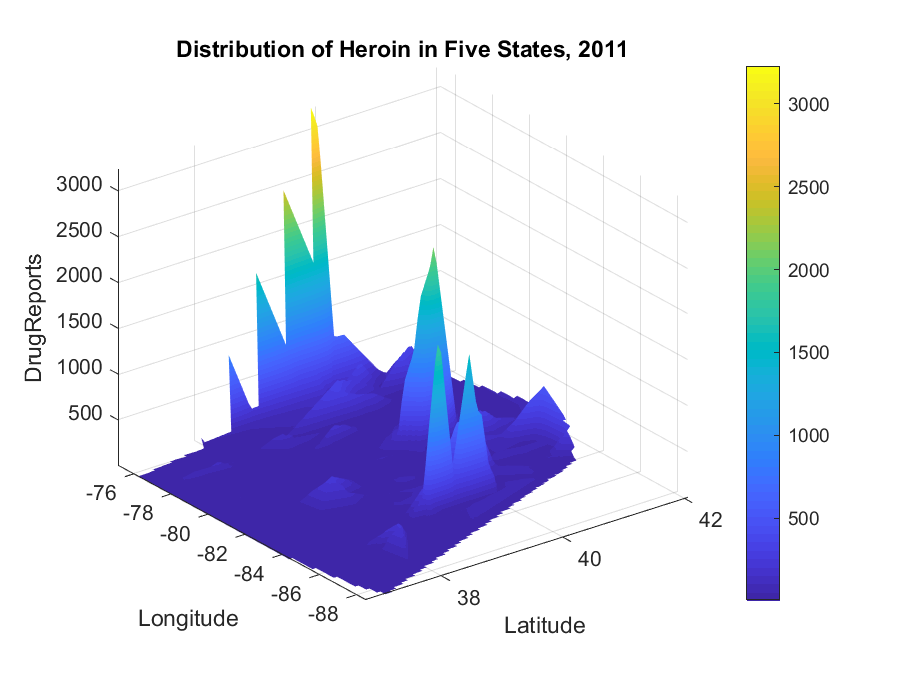
\includegraphics[width=0.7\textwidth]{./pictureb/Herion2011.eps}}
  \caption{Distribution of heroin cases in five states, 2011}\label{fighe11}
\end{figure}
%=============================================
%=====图片格式:eps或者pdf=========================
\begin{figure}[H]
  \centering{
  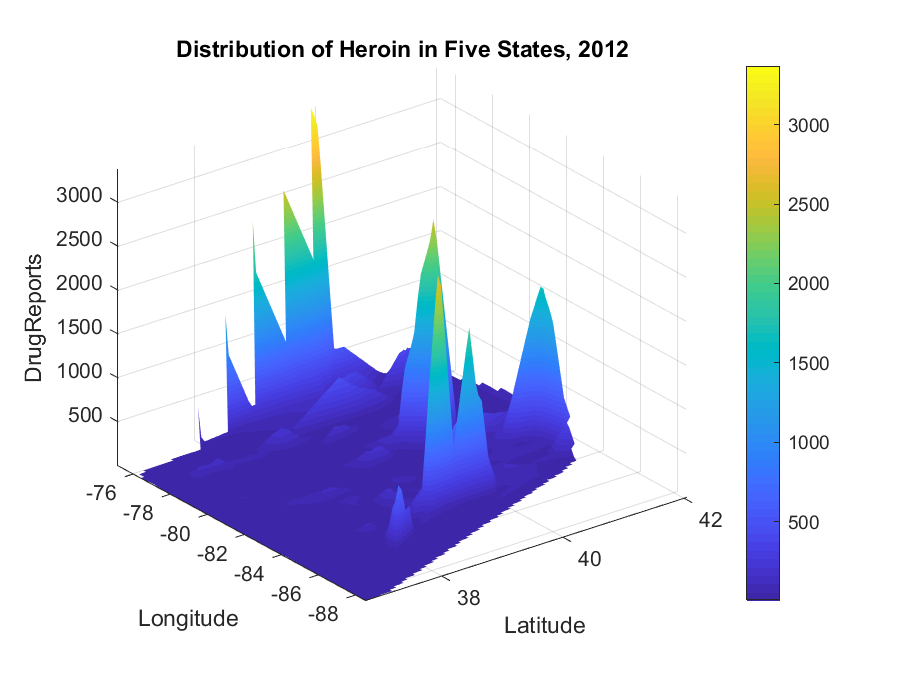
\includegraphics[width=0.7\textwidth]{./pictureb/Herion2012.eps}}
  \caption{Distribution of heroin cases in five states, 2012}\label{fighe12}
\end{figure}
%=============================================
%=====图片格式:eps或者pdf=========================
\begin{figure}[H]
  \centering{
  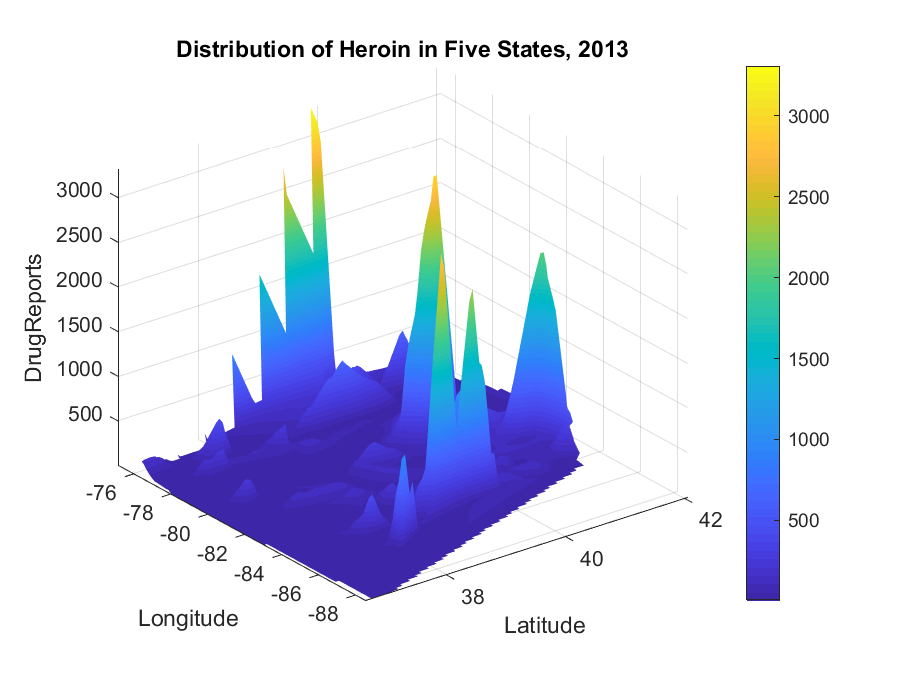
\includegraphics[width=0.55\textwidth]{./pictureb/Herion2013.eps}}
  \caption{Distribution of heroin cases in five states, 2013}\label{fighe13}
\end{figure}
%=============================================
%=====图片格式:eps或者pdf=========================
\begin{figure}[H]
  \centering{
  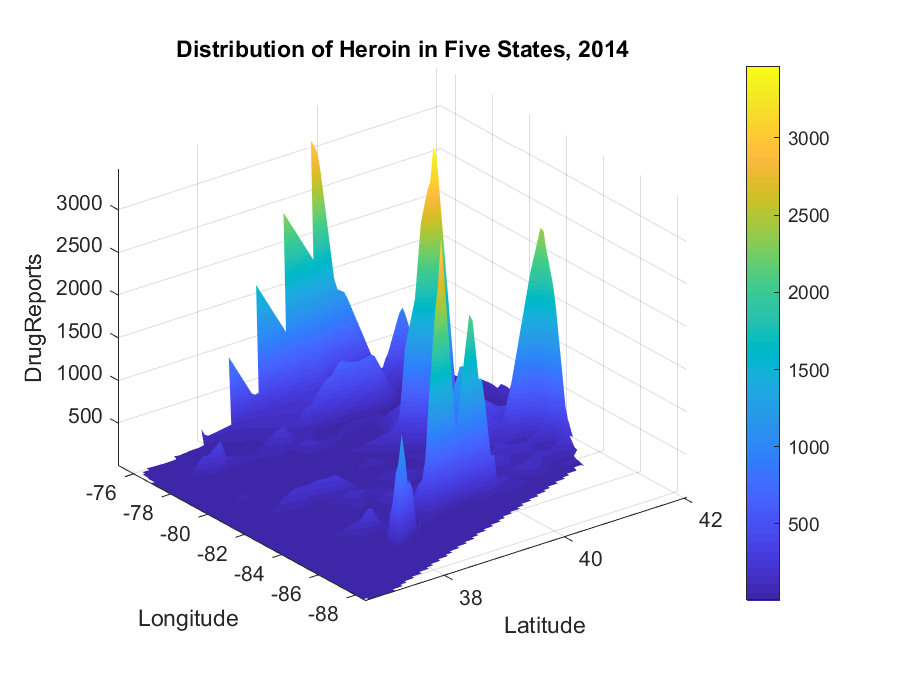
\includegraphics[width=0.55\textwidth]{./pictureb/Herion2014.eps}}
  \caption{Distribution of heroin cases in five states, 2014}\label{fighe14}
\end{figure}
%=============================================
%=====图片格式:eps或者pdf=========================
\begin{figure}[H]
  \centering{
  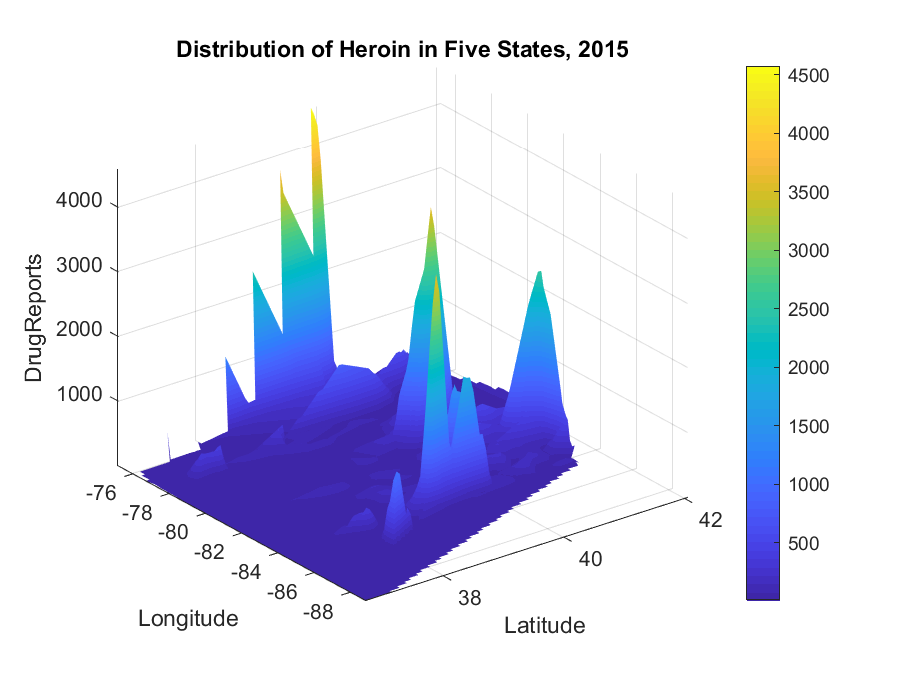
\includegraphics[width=0.55\textwidth]{./pictureb/Herion2015.eps}}
  \caption{Distribution of heroin cases in five states, 2015}\label{fighe15}
\end{figure}
%=============================================
%=====图片格式:eps或者pdf=========================
\begin{figure}[H]
  \centering{
  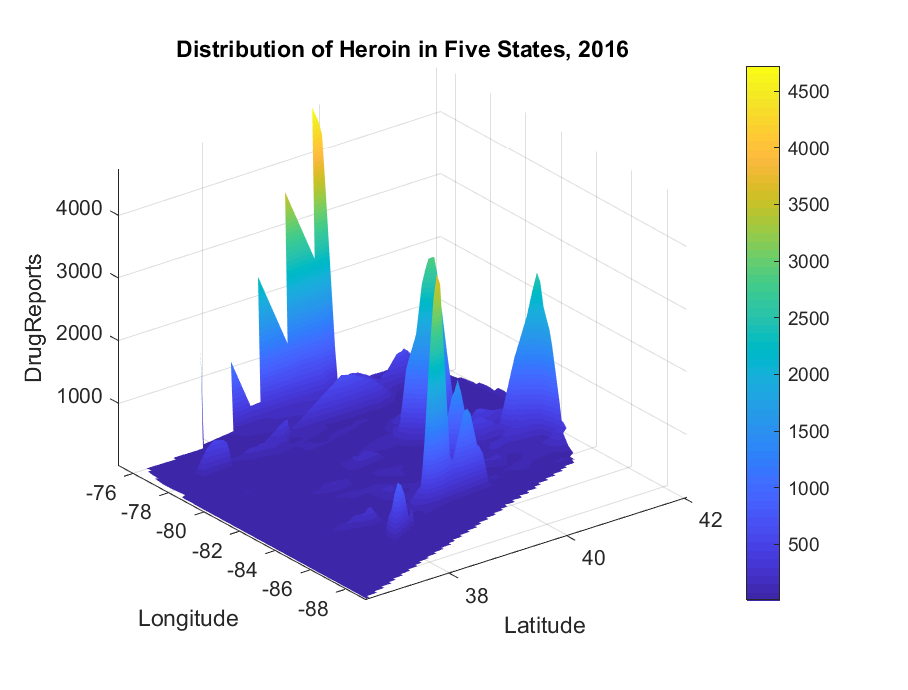
\includegraphics[width=0.5\textwidth]{./pictureb/Herion2016.eps}}
  \caption{Distribution of heroin cases in five states, 2016}\label{fighe16}
\end{figure}
%=============================================

The figures for the distribution of synthetic opioids cases in five states from 2010 to 2017 are shown below.

%=====图片格式:eps或者pdf=========================
\begin{figure}[H]
  \centering{
  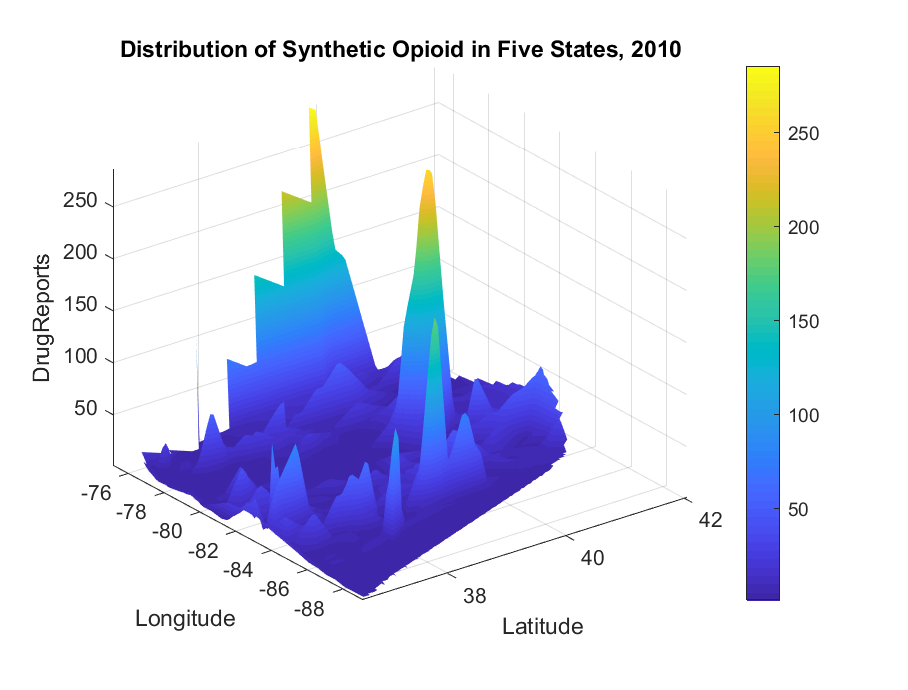
\includegraphics[width=0.5\textwidth]{./pictureb/Opioids2010.eps}}
  \caption{Distribution of synthetic opioids cases in five states, 2010}
  \label{figop10}
\end{figure}
%=============================================
%=====图片格式:eps或者pdf=========================
\begin{figure}[H]
  \centering{
  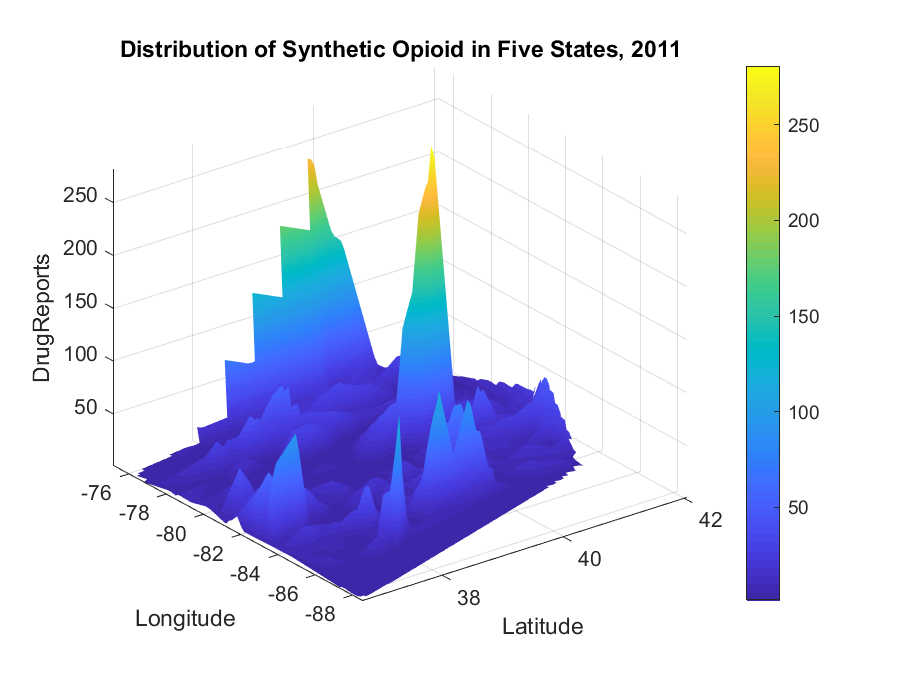
\includegraphics[width=0.5\textwidth]{./pictureb/Opioids2011.eps}}
  \caption{Distribution of synthetic opioids cases in five states, 2011}
  \label{figop11}
\end{figure}
%=============================================
%=====图片格式:eps或者pdf=========================
\begin{figure}[H]
  \centering{
  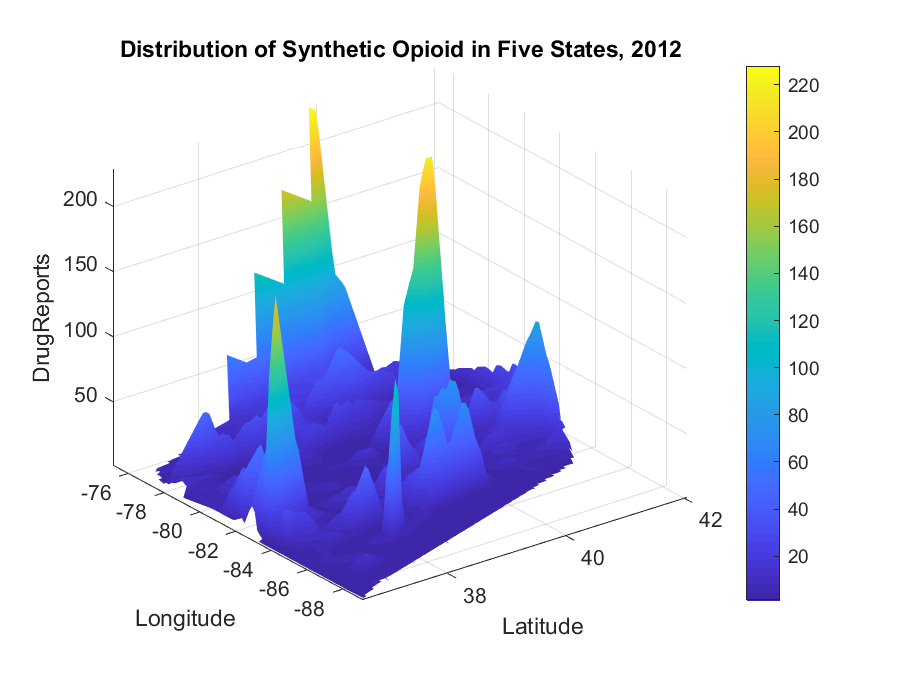
\includegraphics[width=0.55\textwidth]{./pictureb/Opioids2012.eps}}
  \caption{Distribution of synthetic opioids cases in five states, 2012}
  \label{figop12}
\end{figure}
%=============================================
%=====图片格式:eps或者pdf=========================
\begin{figure}[H]
  \centering{
  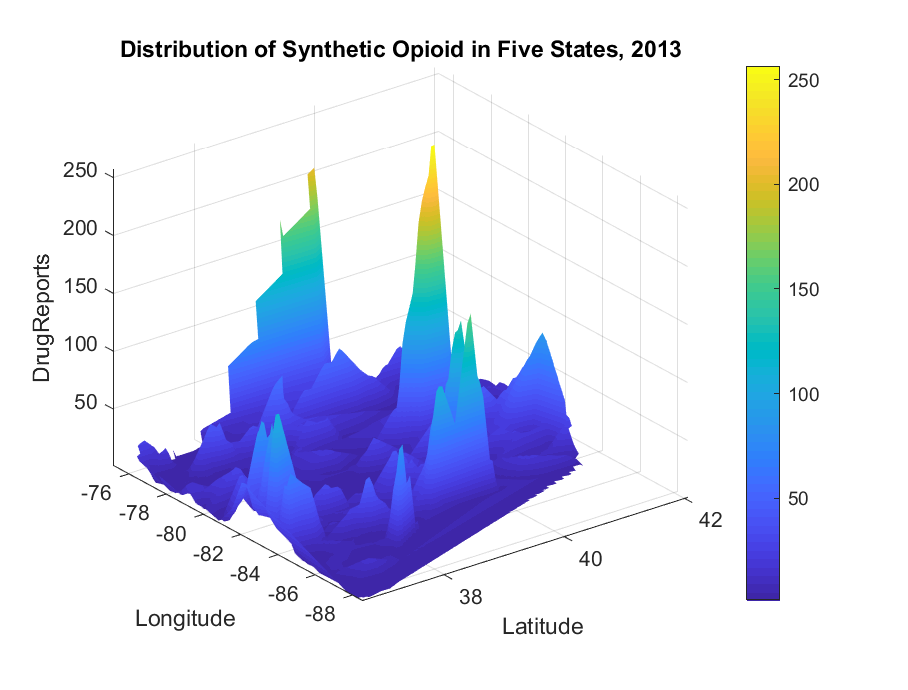
\includegraphics[width=0.55\textwidth]{./pictureb/Opioids2013.eps}}
  \caption{Distribution of synthetic opioids cases in five states, 2013}
  \label{figop13}
\end{figure}
%=============================================
%=====图片格式:eps或者pdf=========================
\begin{figure}[H]
  \centering{
  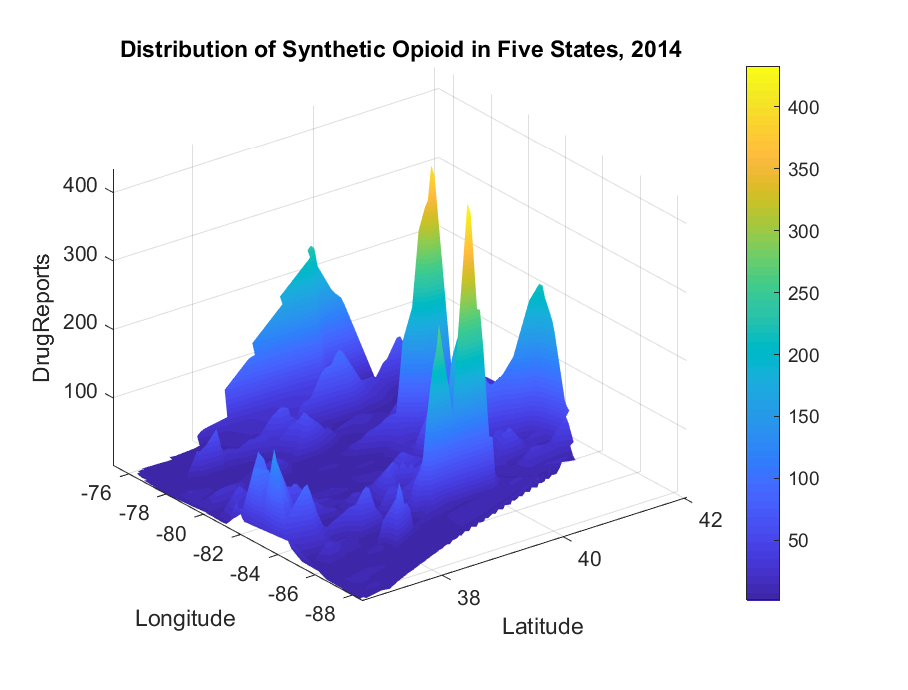
\includegraphics[width=0.55\textwidth]{./pictureb/Opioids2014.eps}}
  \caption{Distribution of synthetic opioids cases in five states, 2014}
  \label{figop14}
\end{figure}
%=============================================
%=====图片格式:eps或者pdf=========================
\begin{figure}[H]
  \centering{
  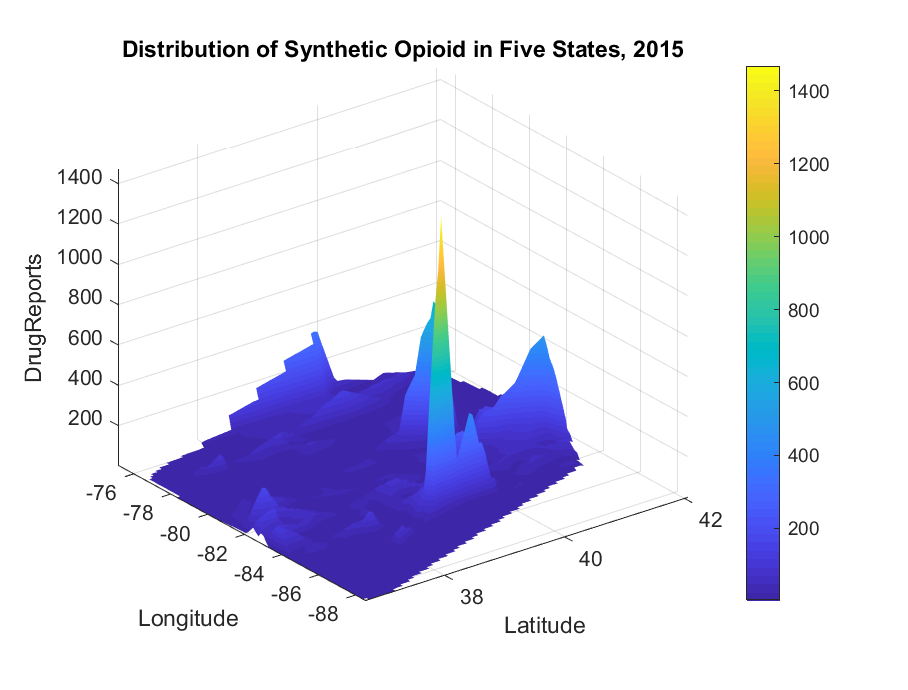
\includegraphics[width=0.55\textwidth]{./pictureb/Opioids2015.eps}}
  \caption{Distribution of synthetic opioids cases in five states, 2015}
  \label{figop15}
\end{figure}
%=============================================
%=====图片格式:eps或者pdf=========================
\begin{figure}[H]
  \centering{
  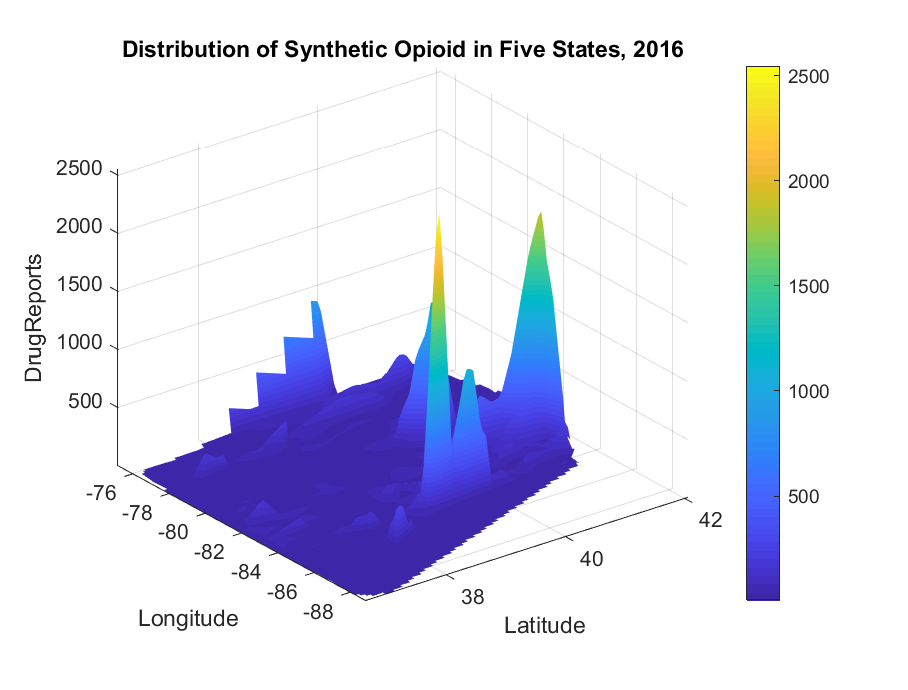
\includegraphics[width=0.55\textwidth]{./pictureb/Opioids2016.eps}}
  \caption{Distribution of synthetic opioids cases in five states, 2016}
  \label{figop16}
\end{figure}
%=============================================
%=====图片格式:eps或者pdf=========================
\begin{figure}[H]
  \centering{
  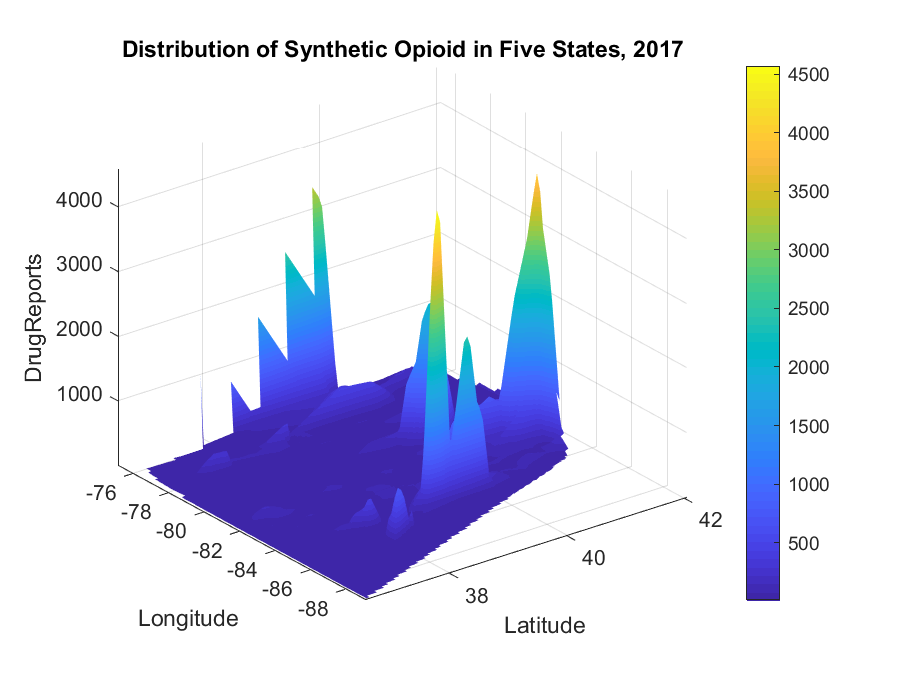
\includegraphics[width=0.55\textwidth]{./pictureb/Opioids2017.eps}}
  \caption{Distribution of synthetic opioids cases in five states, 2017}
  \label{figop17}
\end{figure}
%=============================================


\section{Codes}

Here are programs used for our models.\\

\textbf{\textcolor[rgb]{0.98,0.00,0.00}{Input matlab source:}}
\lstinputlisting[language=Matlab]{./code/mcm_datapro_part1_opioids.m}

\textbf{\textcolor[rgb]{0.98,0.00,0.00}{Input matlab source:}}
\lstinputlisting[language=Matlab]{./code/MCM_C_Part3.m}

\end{appendices}
\end{document}
